\chapter{Espacios Euclídeos}

\begin{definicion}[Espacios euclídeos]
    Diremos que un espacio afín $\bb{E}$ es euclídeo si $\vec{\bb{E}}$ está dotado de la estructura euclídea.
    Es decir, $(\vec{\bb{E}},~\langle,\rangle)$ es un espacio vectorial euclídeo dotado de una aplicación producto escalar.
\end{definicion}

\begin{definicion}
    Sea $\bb{E}$ un espacio euclídeo. Un sistema de referencia $\cc{R}=\{p_o,\cc{B}\}$ de $\bb{E}$ diremos que es
    \ul{euclídeo}, rectangular o ortonormal, si $\cc{B}$ es una base ortonormal.
\end{definicion}

Introducimos el concepto intuitivo de distancia entre dos puntos de un espacio euclídeo.
\begin{definicion}[Distancia]
    Sea $\bb{E}$ un espacio euclídeo. Definimos la aplicación distancia en $\bb{E}\times \bb{E}$ como:
    \Func{d}{\bb{E}\times \bb{E}}{\bb{R}}{(p,q)}{d(p,q)=\|\vec{pq}\|=\sqrt{\langle\vec{pq},\vec{pq}\rangle}}
\end{definicion}

Tenemos que la aplicación anterior es, efectivamente, una distancia, ya que:
\begin{enumerate}
    \item $d(p,q)\geq 0~~\forall p,q\in \bb{E}$. Además, $d(p,q)=0\Longleftrightarrow p=q$.
    \item $d(p,q)=d(q,p)~~\forall p,q\in \bb{E}$.
    \item $d(p,q)\leq d(p,r) + d(r,q)~~\forall p,q,r\in \bb{E}$.
\end{enumerate}


\section{Ortogonalidad}
\begin{definicion}
    Sean $S,T$ dos subespacios afines de $\bb{E}$ espacio euclídeo. Entonces, diremos que $S$ y $T$ son perpendiculares (o ortogonales), notado por $S\perp T$, si y solo si:
    \begin{equation*}
        S\perp T \Longleftrightarrow \vec{S}\perp \vec{T}
    \end{equation*}
\end{definicion}

\begin{teo}
    Sea $\bb{E}$ un espacio euclídeo, y sea $S$ un subespacio afín de $\bb{E}$. Entonces, $\forall q\in \bb{E}$, $\exists_1~ T$ subespacio afín de $\bb{E}$ verificando:
    \begin{enumerate}
        \item $q\in T$,
        \item $T\perp S$,
        \item $\dim T + \dim S = n=\dim \bb{E}$.
    \end{enumerate}
    Dicho subespacio $T$ se denomina \ul{subespacio afín ortogonal a $S$ por $q$}, y se notará por $S_q^\perp=q+\vec{S}^\perp$.
\end{teo}
\begin{proof}
    Consideramos $\vec{S}$, y sabemos que $\vec{S}^\perp$ es el único subespacio vectorial de $\vec{\bb{E}}$
    con $n=\dim \vec{S}+\dim \vec{S}^\perp$ que verifica $\vec{S}\perp \vec{S}^\perp$.

    Consideramos $T=q+\vec{S}^\perp$. Entonces, $T$ es un subespacio afín de $\bb{E}$, ya que $\vec{S}^\perp$ es un subespacio vectorial de $\vec{\bb{E}}$.
    Además, $q\in T$, ya que $q\in q+\vec{S}^\perp$. Por último, tenemos que $\vec{T}=\vec{S}^\perp$, por lo que $T\perp S$. Por tanto, $T$ cumple las tres condiciones.
    
    Tenemos por tanto demostrada la existencia. La unicidad se tiene de forma directa, ya que $\vec{S}^\perp$ es único. Por tanto, para cada $q\in \bb{E}$, tenemos que $T$ es único.
\end{proof}


Una vez introducido el concepto de subespacio ortogonal, incluimos las proyecciones y simetrías ortogonales,
que serán las que mayoritariamente empleemos.
\begin{definicion}[Proyección ortogonal]
    Sea $\cc{A}$ un espacio afín, y sea $S=p+\vec{S}$ un subespacio afín de $\cc{A}$.
    Entonces, definimos la proyección ortogonal respecto de $S$ como la proyección en
    $S$ paralela a $S_p^\perp$:
    \Func{\pi_{S}^\perp}{\cc{A}}{S}{q}{\pi_{S,S_p^\perp}(q) = p + \pi_{\vec{S}}(\vec{pq})}

    Hemos de tener en cuenta que $\pi_{S}^\perp$ también se podrá notar como $\pi_{S}$.
\end{definicion}

\begin{definicion}[Simetría ortogonal]
    Sea $\cc{A}$ un espacio afín, y sea $S=p+\vec{S}$ un subespacio afín de $\cc{A}$.
    Entonces, definimos la simetría ortogonal respecto de $S$ como la simetría en
    $S$ paralela a $S_p^\perp$:
    \Func{\sigma_{S}^\perp}{\cc{A}}{S}{q}{\sigma_{S,S_p^\perp}(q) = p + \sigma_{\vec{S}}(\vec{pq})}

    Hemos de tener en cuenta que $\sigma_{S}^\perp$ también se podrá notar como $\sigma_{S}$.
\end{definicion}


\section{Distancia}

Una vez definida la distancia entre dos puntos, podemos definir la distancia entre subespacios afines de forma general.
\begin{definicion}
    Sea $\bb{E}$ un espacio euclídeo, y sean $S,T$ dos subespacios euclídeos de $\bb{E}$. Entonces, se define la distancia entre $S$ y $T$ como:
    \begin{equation*}
        d(S,T) = \inf\{d(p,q)\mid p\in S,~q\in T\}
    \end{equation*}
\end{definicion}

Veamos los siguientes dos teoremas, que nos facilitan el cálculo de la distancia entre dos subespacios afines:
\begin{teo}\label{teo:existencia_vector_ortogonal}
    Sea $\bb{E}$ un espacio euclídeo, y sean $S=p+\vec{S}$ y $T=q+\vec{T}$ dos subespacios euclídeos de $\bb{E}$.

    Entonces, $\exists p_0\in S,~ q_0\in T$ tal que $\vec{p_0q_0}\in \vec{S}^\perp\cap \vec{T}^\perp = (\vec{S} + \vec{T})^\perp$.


    Además, se tiene que $p_0,q_0$ son únicos si, y solo si, $\vec{S}\cap \vec{T}=\{0\}$.
\end{teo}
\begin{proof}
    Consideramos $\vec{pq}\in \vec{\bb{E}}$. Tenemos que $\vec{\bb{E}}=(\vec{S}+\vec{T}) \oplus (\vec{S}+\vec{T})^\perp$. Por tanto, tenemos que $\vec{pq}=u+v+w$, con $u\in \vec{S}$, $v\in \vec{T}$, $w\in (\vec{S}+\vec{T})^\perp$. Definimos $q_0=q-v\in T$, $p_0= p+u\in S$, y tenemos que:
    \begin{equation*}
        w = \vec{pq} - u -v = q-p-u-v=q_0-p_0=\vec{p_0q_0} \in (\vec{S} + \vec{T})^\perp = \vec{S}^\perp\cap \vec{T}^\perp
    \end{equation*}

    Respecto a la unicidad, tenemos que $p_0, q_0$ son únicos si $u,v$ son únicos. Esto se da si y solo si $\vec{S}\oplus \vec{T}$, y esto se da si y solo si $\vec{S}\cap \vec{T}=\{0\}$.
\end{proof}

\begin{coro}\label{coro:dist_ortogonal}
    Sea $\bb{E}$ un espacio euclídeo, y sean $S=p+\vec{S}$ y $T=q+\vec{T}$ dos subespacios euclídeos de $\bb{E}$.

    Se tiene que $\exists p_0\in S,~ q_0\in T$ tal que $\vec{p_0q_0}\in \vec{S}^\perp\cap \vec{T}^\perp$ cumpliendo que:
    \begin{equation*}
        d(S,T)=d(p_0,q_0)
    \end{equation*}
\end{coro}
\begin{proof}
    La demostración de la existencia se ha visto en el teorema anterior. Una vez demostrada la existencia, veamos que cumplen la relación de las distancias. Sean $a\in S, b\in T$. Veamos que $d(p_0,q_0)\leq d(a,b)$:
    \begin{multline*}
        d^2(a,b)=\|\vec{ab}\|^2= \langle\vec{ab},\vec{ab}\rangle = 
        \langle\vec{ap_0}+\vec{p_0q_0}+\vec{q_0b},\vec{ap_0}+\vec{p_0q_0}+\vec{q_0b}\rangle = \\=
        \|\vec{ap_0}+\vec{q_0b}\|^2 + \|\vec{p_0q_0}\|^2 + \cancel{2\langle\vec{ap_0}+\vec{q_0b},\vec{p_0q_0}\rangle} \geq \|\vec{p_0q_0}\|^2 = d^2(p_0,q_0)
    \end{multline*}
    donde $\langle\vec{ap_0}+\vec{q_0b},\vec{p_0q_0}\rangle=0$, ya que $\vec{ap_0}\in \vec{S}$, $\vec{q_0b}\in \vec{T}$, y $\vec{p_0q_0}\in \vec{S}^\perp,\vec{T}^\perp$.

    Por tanto,
    \begin{equation*}
        d(p_0,q_0)\leq d(a,b) \qquad \forall a\in S~b\in T
    \end{equation*}

    Por tanto, tenemos que $d(p_0,q_0)$ es un minorante de $\{d(p,q)\mid p\in S,~q\in T\}$. Además, como $p_0\in S$, $q_0\in T$, tenemos que pertenece al conjunto. Por tanto, no solo es minorante sino que también es el mínimo, por lo que $d(p_0,q_0)$ es el mínimo y, por consecuente, es el ínfimo.
\end{proof}

\begin{coro}
    Sea $\bb{E}$ un espacio euclídeo, y sean $S,T$ dos subespacios afines de $\bb{E}$. Entonces, tenemos que:
    \begin{equation*}
        d(S,T)=0 \Longleftrightarrow S\cap T \neq \emptyset
    \end{equation*}
\end{coro}
\begin{proof}\
\begin{description}
    \item[$\Longrightarrow)$] Tenemos que $\exists p_0\in S,~ q_0\in T$ tal que $\vec{p_0q_0}\in \vec{S}^\perp\cap \vec{T}^\perp$ cumpliendo que:
    \begin{equation*}
        d(S,T)=d(p_0,q_0)
    \end{equation*}

    Entonces, si $d(S,T)=d(p_0,q_0)=0$, entonces $p_0=q_0$, por lo que $S\cap T\neq \emptyset$.

    \item[$\Longleftarrow)$] Tenemos que $d(S,T)=\inf\{d(p,q)\mid p\in S,~q\in T\}$. Entonces, sea $p_0\in S\cap T$. Entonces, $d(p_0,p_0)=0=d(S,T)$.
\end{description}
\end{proof}

\begin{coro}
    Sea $\bb{E}$ un espacio euclídeo, y sea $S$ un subespacio afín de $\bb{E}$ y $q_0\in \bb{E}$. Entonces, se tiene que:
    \begin{equation*}
        d(S,q_0)=d(q_0, \pi_S(q_0))
    \end{equation*}
\end{coro}
\begin{proof}
    Como hemos visto, $\exists p_0\in S$ tal que $\vec{p_0q_0}\in \vec{S}^\perp$ cumpliendo que:
    \begin{equation*}
        d(S,q_0)=d(p_0,q_0)
    \end{equation*}

    Veamos ahora que $p_0=\pi_S(q_0)$. Tenemos que:
    \begin{equation*}
        \pi_S(q_0) = p_0 + \pi_{\vec{S}}(\vec{p_0q_0}) = p_0 + \vec{0} = p_0
    \end{equation*}
    donde he usado que, como $\vec{p_0q_0}\in \vec{S}^\perp$, entonces $\pi_{\vec{S}}(\vec{p_0q_0})=\vec{0}$.
    Por tanto, tenemos que:
    \begin{equation*}
        d(S,q_0)=d(p_0,q_0)=d(q_0, \pi_S(q_0))
    \end{equation*}
\end{proof}

\begin{ejemplo}
    Sea $\bb{R}^3$ espacio euclídeo, y consideramos $$S= (1,0,1)+\cc{L}\{(1,1, 0)\}\qquad \qquad T= (1,1,0)+\cc{L}\{(-1,1,0)\}$$
    rectas euclídeas de $\bb{R}^3$. Calcular $d(S,T)$.\\

    Un punto arbitrario de la recta $S$ es $p=(1+\alpha, \alpha, 1)$, y uno de la recta $T$ es $q=(1-\beta, 1+\beta, 0)$ para ciertos $\alpha,\beta\in \bb{R}$. Por tanto, $\vec{qp}=(\alpha + \beta, \alpha-\beta-1, 1)$.

    Como $\vec{qp}\in \vec{S}^\perp$, entonces:
    \begin{equation*}
        \langle (\alpha+\beta, \alpha-\beta-1, 1), (1,1,0)\rangle = 0 = 2\alpha-1 \Longrightarrow \alpha = \frac{1}{2}
    \end{equation*}
    
    Como $\vec{qp}\in \vec{T}^\perp$, entonces:
    \begin{equation*}
        \langle (\alpha+\beta, \alpha-\beta-1, 1), (-1,1,0)\rangle = 0 = -2\beta-1 \Longrightarrow \beta = -\frac{1}{2}
    \end{equation*}

    Por tanto, $p=(\nicefrac{3}{2},\nicefrac{1}{2}, 1)$, $q=(\nicefrac{3}{2}, \nicefrac{1}{2}, 0)$. Entonces,
    \begin{equation*}
        d(S,T)=d(p,q) = \|q-p\| = \|(0,0,-1)\| = 1
    \end{equation*}
\end{ejemplo}

\section{Ángulos}
En esta sección trataremos el concepto de ángulo entre subespacios afines. Es importante notar que
este no se define para cualquier par de subespacios afines, sino que se define en casos concretos, como veremos.

\subsubsection{Ángulo entre dos rectas}
El primer caso particular que trataremos es el ángulo entre dos rectas.
\begin{definicion}[Ángulo entre dos rectas]
    Sea $\bb{E}$ un espacio euclídeo. Consideramos dos rectas secantes $r_1=p_1 + \cc{L}\{v_1\}$, $r_2=p_2 + \cc{L}\{v_2\}$. Definimos el ángulo entre dos secantes como:
    \begin{equation*}
        \measuredangle(r_1,r_2)
        := \min\{\measuredangle(v_1,v_2), \measuredangle(v_1,-v_2)\}
    \end{equation*}
    \begin{figure}[H]
        \centering
        \begin{tikzpicture}[scale=0.6]
            % Define los puntos de las rectas
            \coordinate (r1_ini) at (-4,-2);
            \coordinate (r1_fin) at (4,2);
            \coordinate (r2_ini) at (-4,2);
            \coordinate (r2_fin) at (4,-2);

            \coordinate (O) at (0,0);
            \coordinate (v_1) at (2,1);
            \coordinate (v_2) at (2,-1);
        
            % Dibuja las rectas
            \draw (r1_ini) -- (r1_fin);
            \draw (r2_ini) -- (r2_fin);

            % Etiqueta las rectas
            \node[right] at (r1_fin) {$r_1$};
            \node[right] at (r2_fin) {$r_2$};

            % Dibuja los vectores directores
            \draw[-stealth, blue] (O) -- node[above]{$v_1$} (v_1);
            \draw[-stealth, red] (O) -- node[below]{$v_2$} (v_2);

            \tkzMarkAngle[size=0.5](v_2,O,v_1);
            \tkzLabelAngle[pos=0.8](v_2,O,v_1){$\alpha$};
        \end{tikzpicture}
        \caption{Vista gráfica del ángulo $\alpha$ entre dos rectas.}
    \end{figure}
\end{definicion}
Notemos que la definición con el mínimo se debe a que dos rectas secantes generan dos ángulos, y buscamos el menor ángulo entre ellas.

De esta definición se deduce directamente el siguiente resultado:
\begin{prop}
    Sea $\bb{E}$ un espacio euclídeo. Consideramos dos rectas paralelas $r_1=p_1 + \cc{L}\{v\}$, $r_2=p_2 + \cc{L}\{v\}$, y $T=p_T + \cc{L}\{v_p\}$ secante a ambas. Entonces:
    \begin{equation*}
        \measuredangle(T,r_2)
        = \measuredangle(T,r_1)
    \end{equation*}
    \begin{figure}[H]
        \centering
        \begin{tikzpicture}[scale=0.6]
            % Define los puntos de las rectas
            \coordinate (r1_ini) at (-4,-1);
            \coordinate (r1_fin) at (4,-1);
            \coordinate (r2_ini) at (-4,1);
            \coordinate (r2_fin) at (4,1);
            \coordinate (T_ini) at (-4,-2);
            \coordinate (T_fin) at (4,2);

            \coordinate (O) at (0,0);
            \coordinate (C_2) at (2,1);
            \coordinate (C_1) at (-2,-1);
        
            % Dibuja las rectas
            \draw (r1_ini) -- (r1_fin);
            \draw (r2_ini) -- (r2_fin);
            \draw (T_ini) -- (T_fin);

            % Etiqueta las rectas
            \node[right] at (r1_fin) {$r_1$};
            \node[right] at (r2_fin) {$r_2$};
            \node[right] at (T_fin) {$T$};

            \tkzMarkAngle[size=0.8](r1_fin,C_1,T_fin);
            \tkzMarkAngle[size=0.8](r2_fin,C_2,T_fin);
            \tkzLabelAngle[pos=1.3](r1_fin,C_1,T_fin){$\alpha$};
            \tkzLabelAngle[pos=1.3](r2_fin,C_2,T_fin){$\alpha$};
        \end{tikzpicture}
    \end{figure}
\end{prop}
\begin{proof}
    Tenemos que:
    \begin{equation*}
        \measuredangle(T,r_2) = \min\{\measuredangle(v,v_T), \measuredangle(v,-v_T)\}
        = \measuredangle(T,r_1)
    \end{equation*}
\end{proof}

\subsubsection{Ángulo entre recta e hiperplano}
A continuación trataremos el caso particular de un hiperplano y una recta. No obstante, para ello hemos de recordar el concepto de vector normal,
introducido en Geometría II.
\begin{definicion}[Vector normal]
    Sea $\vec{\bb{E}}$ un espacio vectorial euclídeo, y sea $\vec{H}$ un hiperplano de $\vec{\bb{E}}$. Entonces, diremos que $v_H \in \vec{\bb{E}}$ es un vector normal a $\vec{H}$ si y solo si:
    \begin{equation*}
        v_H\in  \vec{H}^\perp
    \end{equation*}
    Notemos que $v_H$ es único salvo factores de proporcionalidad.
\end{definicion}
\begin{definicion}
    Sea $\bb{E}$ un espacio euclídeo, y sea $H$ un hiperplano de $\bb{E}$. Entonces, diremos que $v_H \in \vec{\bb{E}}$ es un vector normal a $H$ si y solo si $v$
    es un vector normal a $\vec{H}$.
\end{definicion}
\begin{prop}
    Sea $\vec{\bb{E}}$ un espacio vectorial euclídeo, y sea $v\in \vec{\bb{E}}$. Entonces, existe un único hiperplano $\vec{H}$ de $\vec{\bb{E}}$
    tal que $v$ es un vector normal a $\vec{H}$.
\end{prop}
\begin{proof}
    Sea $n=\dim \vec{\bb{E}}$. Ampliamos $\{v\}$ a una base ortonormal de $\vec{\bb{E}}$, $\cc{B}=\{v,v_2,\dots,v_n\}$.
    Entonces, $\vec{H}=\cc{L}\{v_2,\dots,v_n\}$ es un hiperplano de $\vec{\bb{E}}$. Además, por ser la base ortonormal, tenemos que $v\in \vec{H}^\perp$, es decir,
    $v$ es un vector normal a $\vec{H}$.

    Por último, veamos que $\vec{H}$ es único. Supongamos que $\vec{H}'$ es otro hiperplano de $\vec{\bb{E}}$ tal que $v$ es un vector normal a $\vec{H}'$.
    Entonces, $\vec{H}'=\cc{L}\{v_2',\dots,v_n'\}$, con $\cc{B}'=\{v,v_2',\dots,v_n'\}$ base ortonormal de $\vec{\bb{E}}$. Entonces, $\vec{H}=\vec{H}'$.
\end{proof}

\begin{definicion}[Ángulo entre recta e hiperplano]
    Sea $\bb{E}$ un espacio euclídeo, y sean $r=p+\cc{L}\{v\}$ una recta y $H$ un hiperplano de $\bb{E}$ con $v_H\in \vec{\bb{E}}$ vector normal a $H$.
    Entonces, definimos el ángulo entre la recta y el hiperplano como:
    \begin{equation*}
        \measuredangle(r,H) := \frac{\pi}{2} - \min\{\measuredangle(v,v_H), \measuredangle(v,-v_H)\}
    \end{equation*}
\end{definicion}
\begin{figure}[H]
    \centering
    \begin{tikzpicture}
        % Definir los vértices del romboide
        \coordinate (A) at (0,0);
        \coordinate (B) at (2,1);
        \coordinate (C) at (8,1);
        \coordinate (D) at  (6,0);
    
        \coordinate (T_arr) at  (6,3);
        \coordinate (T_ab) at  (3.2,-0.5);
        
        \coordinate (p_0) at  (4,0.5);
        \coordinate (v) at  (5, 1.75);
        \coordinate (v_H) at  (4, 2);
        \coordinate (dot_init) at  (3, 0.5);
        \coordinate (dot_fin) at  (5, 0.5);
    
        % Dibujar el romboide
        \draw[gray, thick] (A) -- (B) -- (C) -- (D) -- cycle;
        \node[above] at (A) {$H$};
  
        
        % Dibujar la recta r
        \draw (p_0) -- (T_arr) node[above]{$r$};
        \draw[dotted] (3.6,0) -- (p_0);
        \draw (3.6, 0) -- (T_ab);

        % Dibujar el vector director de r
        \fill[] (p_0) circle (2pt);
        \fill[red] (v) circle (1pt);
        \draw[-stealth, red] (p_0) -- (v) node[right] {$v$};

        % Dibujar el vector normal a H
        \fill[blue] (v_H) circle (1pt);
        \draw[-stealth, blue] (p_0) -- (v_H) node[right] {$v_H$};


        % Marca de ángulo recto en V_h
        \draw[dotted]  (dot_init) -- (dot_fin);
        \tkzMarkRightAngle[size=0.2](v_H,p_0,dot_init);
        
        % Marca del ángulo entre v y v_h
        \tkzMarkAngle[size=0.6](v,p_0,v_H);
        \tkzLabelAngle[pos=0.8](v,p_0,v_H){$\alpha$};

        % Marca del ángulo entre v y H
        \tkzMarkAngle[size=0.9, teal](dot_fin,p_0,v);
        \tkzLabelAngle[pos=1.5, teal](dot_fin,p_0,v){$\frac{\pi}{2} - \alpha$};
    \end{tikzpicture}
    \caption{Representación gráfica del ángulo entre una recta y un hiperplano.}
\end{figure}



\subsubsection{Ángulo entre dos hiperplanos}

El tercer caso particular que trataremos es el ángulo entre dos hiperplanos.
\begin{definicion}[Ángulo entre dos hiperplanos]
    Sea $\bb{E}$ un espacio euclídeo, y sean $H_1, H_2$ dos hiperplanos de $\bb{E}$ con $v_{1}\in \vec{\bb{E}}$ vector normal a $H_1$ y $v_{2}\in \vec{\bb{E}}$ vector normal a $H_2$.
    Entonces, definimos el ángulo entre dos dos hiperplanos como:
    \begin{equation*}
        \measuredangle(H_1,H_2) = \min\{\measuredangle(v_1,v_2), \measuredangle(v_1,-v_2)\}
    \end{equation*}
\end{definicion}
\begin{comment}
\begin{figure}[H]
    \centering
    \begin{tikzpicture}
        % Definir los vértices de H_1
        \coordinate (A) at (0,0);
        \coordinate (B) at (2,1);
        \coordinate (C) at (8,1);
        \coordinate (D) at  (6,0);

        % Definir los vértices de H_2
        \coordinate (A') at (0,0);
        \coordinate (B') at (2,1);
        \coordinate (C') at (8,1);
        \coordinate (D') at  (6,0);
    
        \coordinate (T_arr) at  (6,3);
        \coordinate (T_ab) at  (3.2,-0.5);
        
        \coordinate (p_0) at  (4,0.5);
        \coordinate (v) at  (5, 1.75);
        \coordinate (v_H) at  (4, 2);
        \coordinate (dot_init) at  (3, 0.5);
        \coordinate (dot_fin) at  (5, 0.5);
    
        % Dibujar el romboide
        \draw[gray, thick] (A) -- (B) -- (C) -- (D) -- cycle;
        \node[above] at (A) {$H$};
  
        
        % Dibujar la recta r
        \draw (p_0) -- (T_arr) node[above]{$r$};
        \draw[dotted] (3.6,0) -- (p_0);
        \draw (3.6, 0) -- (T_ab);

        % Dibujar el vector director de r
        \fill[] (p_0) circle (2pt);
        \fill[red] (v) circle (1pt);
        \draw[-stealth, red] (p_0) -- (v) node[right] {$v$};

        % Dibujar el vector normal a H
        \fill[blue] (v_H) circle (1pt);
        \draw[-stealth, blue] (p_0) -- (v_H) node[right] {$v_H$};


        % Marca de ángulo recto en V_h
        \draw[dotted]  (dot_init) -- (dot_fin);
        \tkzMarkRightAngle[size=0.2](v_H,p_0,dot_init);
        
        % Marca del ángulo entre v y v_h
        \tkzMarkAngle[size=0.6](v,p_0,v_H);
        \tkzLabelAngle[pos=0.8](v,p_0,v_H){$\alpha$};

        % Marca del ángulo entre v y H
        \tkzMarkAngle[size=0.9, teal](dot_fin,p_0,v);
        \tkzLabelAngle[pos=1.5, teal](dot_fin,p_0,v){$\frac{\pi}{2} - \alpha$};
    \end{tikzpicture}
    \caption{Representación gráfica del ángulo entre una recta y un hiperplano.}
\end{figure}
% // TODO: Dibujar el ángulo entre dos hiperplanos
\end{comment}

\subsubsection{Ángulo Orientado}
A continuación, recordaremos el concepto de ángulo orientado, introducido en Geometría II. Como podemos ver en la Figura \ref{fig:ProblemaOrientacion}, tenemos que $\cos\alpha = \cos\alpha'$, por lo que la definición de ángulo no orientado no basta para diferenciar ambos ángulos. Por ello, introducimos el concepto de orientación:
\begin{figure}[H]
    \centering
    \begin{tikzpicture}
        % Define los puntos de las rectas
        \coordinate (O) at (0,0);
        \coordinate (O_Dcha) at (3.5,0);
        \coordinate (O_Izq) at (-1,0);
        \coordinate (P) at (3,1.5);
        \coordinate (Q) at (3,-1.5);

        \filldraw (O) circle (2pt);
    
        % Dibuja los vectores
        \draw[-stealth] (O) -- node[above]{$u_1$} (P);
        \draw[-stealth] (O) -- node[below]{$u_2$} (Q);
        \draw[-stealth] (O) -- node[below]{$v$} (O_Dcha);
        \draw[dashed] (O_Izq) -- (O);

        \tkzMarkAngle[size=1cm, red](O_Dcha,O,P)
        \tkzMarkAngle[size=0.8cm, blue](Q,O,O_Dcha)
        \tkzLabelAngle[pos=1.3, red](O_Dcha,O,P){$\alpha$}
        \tkzLabelAngle[pos=1.1, blue](Q,O,O_Dcha){$\alpha$}
    \end{tikzpicture}
    \caption{Representación del problema de los ángulos no orientados.}
    \label{fig:ProblemaOrientacion}
\end{figure}

\begin{definicion}
    Dado $V$ un espacio vectorial, diremos que fijamos una orientación en él al fijar una base $\cc{B}$, y diremos que $V$ es orientado. Dada otra base $\cc{B}'$, diremos que:
    \begin{enumerate}
        \item Tienen la misma orientación (o es positivamente orientada) si $|M(\cc{B}',\cc{B})|>0$.
        \item Tienen orientación contraria (o es negativamente orientada) si $|M(\cc{B}',\cc{B})|<0$.
    \end{enumerate}
\end{definicion}

\begin{teo}
    Sea $V$ un plano euclídeo orientado. Entonces, $\forall u\in V$, $\exists_1 Ju\in V$ tal que $u\perp Ju$, $\|u\| = \|Ju\|$ y la base $\{u,Ju\}$ es positivamente orientada.
\end{teo}
\begin{comment}
\begin{proof}
    Sea la base del plano positivamente orientada $\cc{B} = \{e_1,e_1\}$. Sea $u=(u_1,u_2)_{\cc{B}}$, y sea  $Ju=(x,y)_{\cc{B}}$. Veamos si esos valores de $x,y$ son únicos.

    Como $u\perp Ju$, entonces:
    \begin{equation*}
        \langle u,Ju\rangle = 0 \Longrightarrow u_1x+u_2y = 0
    \end{equation*}

    Como $\|u\| = \|Ju\|$, entonces:
    \begin{equation*}
        \sqrt{u_1^2+u_2^2} = \sqrt{x^2+y^2} \Longrightarrow u_1^2+u_2^2 = x^2+y^2
    \end{equation*}
\end{proof}
\end{comment}

\begin{definicion}
    Dados $u,v\in V$ espacio vectorial euclídeo orientado, definimos el ángulo orientado de $u$ a $v$, notado por $\measuredangle_o(u,v)$, por el único real $\theta\in [0,2\pi[$ tal que:
    \begin{equation*}
        \frac{v}{\|v\|} = \cos\theta \frac{u}{\|u\|} + \sen\theta \frac{Ju}{\|Ju\|}
    \end{equation*}
\end{definicion}

Algunas propiedades que se deducen del ángulo orientado son, $\forall u,v,w\in V$, $\lambda,\mu\in \bb{R}$:
\begin{enumerate}
    \item $\measuredangle_o(u,v) = -\measuredangle_o(v,u)$,
    \item $\measuredangle_o(u,-u) = \pi$,
    \item $\measuredangle_o (u,v) = \measuredangle_o(-u-v)$,
    \item $\measuredangle_o (u,v) = \measuredangle_o(\lambda u, \mu v)$,
    \item $\measuredangle_o (u,v) = \measuredangle_o(u,w) + \measuredangle_o(w,v)$.
\end{enumerate}

Una vez recordados los conceptos de ángulo orientado para espacios vectoriales euclídeos, retomamos los espacios afines euclídeos.
\begin{definicion}
    Sea $\bb{E}$ un espacio euclídeo. Decimos que $\bb{E}$ es orientado si $\vec{\bb{E}}$ tiene fijada una orientación.
\end{definicion}



\section{Isometrías}
\begin{definicion}[Isometrías]
    Sea $f:\bb{E}\to \bb{E}'$ aplicación afín entre espacios euclídeos. Decimos que $f$ es una isometría afín o un movimiento rígido si 
    $$d(p,q)=d(f(p),f(q))\qquad \forall p,q\in \bb{E}$$
\end{definicion}
\begin{ejemplo}
    Sea $\bb{E}$ en espacio euclídeo, y sea $v\in \vec{\bb{E}}$. Entonces, $t_v$ es una isometría. Veámoslo:
    \begin{equation*}
        d(t_v(p), t_v(q))=d(p+v, q+v)=\|q-p\|=\|\vec{pq}\|=d(p,q)
    \end{equation*}
\end{ejemplo}

Es directo pensar que las isometrías afines están relacionadas con las isometrías vectoriales. Veámoslo:
\begin{teo}
    Sea $f:\bb{E}\to \bb{E}'$ aplicación afín entre espacios euclídeos con $\vec{f}$ aplicación lineal asociada. Entonces:
    \begin{center}
        $f$ isometría afín $\Longleftrightarrow$ $\vec{f}$ isometría vectorial 
    \end{center}
\end{teo}
\begin{proof}\
    \begin{description}
        \item[$\Longrightarrow)$] Supongamos que $f$ es una isometría afín. Entonces, 
        $$d(p,q)=d(f(p),f(q))\qquad \forall p,q\in \bb{E}$$

        Como, por definición, $d(p,q)=\langle \vec{pq},\vec{pq}\rangle$, tenemos:
        \begin{equation*}
            \langle \vec{pq}, \vec{pq}\rangle
            = \langle \vec{f(p)f(q)}, \vec{f(p)f(q)}\rangle \qquad \forall p,q\in \bb{E}
        \end{equation*}

        Por ser $f$ una aplicación afín, tenemos que:
        \begin{equation*}
            \langle \vec{pq}, \vec{pq}\rangle
            = \langle \vec{f}(\vec{pq}), \vec{f}(\vec{pq})\rangle  \qquad \forall p,q\in \bb{E}
        \end{equation*}

        Por tanto, queda demostrado que $\vec{f}$ es una isometría.

        \item[$\Longleftarrow)$] Suponemos que $\vec{f}$ es una isometría vectorial. Por tanto,
        \begin{equation*}
            \langle u,v\rangle = \langle \vec{f}(u),\vec{f}(v)\rangle \qquad \forall u,v\in \vec{\bb{E}}
        \end{equation*}

        Como, fijado $p_0\in \bb{E}$, todo vector $v\in \vec{\bb{E}}$ se puede poner como $v=\vec{p_0p}$, con $p\in \bb{E}$, entonces:
        \begin{equation*}
            \langle \vec{p_0p},\vec{p_0q}\rangle = \left\langle \vec{f}(\vec{p_0p}),\vec{f}(\vec{p_0q})\right\rangle \qquad \forall p,q\in {\bb{E}}
        \end{equation*}

        Por ser $\vec{f}$ la aplicación lineal asociada a $f$, tenemos que:
        \begin{equation*}
            \langle \vec{p_0p},\vec{p_0q}\rangle = \left\langle \vec{f(p_0)f(p)},\vec{f(p_0)f(q)}\right\rangle \qquad \forall p,q\in {\bb{E}}
        \end{equation*}

        Usando la norma en $\vec{\bb{E}}$, tenemos:
        \begin{equation*}
            \|\vec{p_0q} - \vec{p_0p}\|^2
            = \|\vec{f(p_0)f(q)} -  \vec{f(p_0)f(p)}\|^2  \qquad \forall p,q\in {\bb{E}}
        \end{equation*}

        Usando la igualdad triangular, tenemos:
        \begin{equation*}
            \|\vec{pq}\|^2
            = \|\vec{f(p)f(q)}\|^2 \Longrightarrow d(p,q)=d(f(p), f(q))  \qquad \forall p,q\in {\bb{E}}
        \end{equation*}

        Por tanto, tenemos que $f$ es una isometría afín.
    \end{description}
\end{proof}

Recordemos el siguiente lema, tratado en Geometría II:
\begin{lema}
    Sea $\varphi:V^n\to V^{'m}$ una isometría entre espacios vectoriales. Entonces, $\varphi$ es inyectiva y lineal.
\end{lema}
\begin{coro}
    Sean $\bb{E},\bb{E}'$ dos espacios euclídeos. Consideramos $f:\bb{E}\to \bb{E}'$ una isometría afín. Entonces, tenemos que $f$ es inyectiva, afín y $\vec{f}$ es una isometría vectorial.
\end{coro}

\section{Clasificación de los movimientos}
Sea $f:\bb{E}^n\to \bb{E}^n$ un movimiento. Tenemos los siguientes tipos de movimientos:
\begin{itemize}
    \item \ul{Directo}: Conserva la orientación. $|\vec{f}|=1$.
    \item \ul{Inverso}: Invierte la orientación. $|\vec{f}|=-1$.
\end{itemize}
Para clasificarlas, partimos de la clasificación de las isometrías vectoriales, vista en Geometría III. Recordemos que una aplicación afín viene determinada por su aplicación lineal asociada y la imagen del origen. Es es debido a que, dados dos espacios afines $\cc{A}$, $\cc{A}'$ y sus respectivos sistemas de referencia $\cc{R}=\{p_0,\cc{B}\}, \cc{R}'=\{p_0',\cc{B}'\}$, entonces:
\begin{equation*}
    f(p)_{\cc{R}'} = f(p_0)_{\cc{R}'} + \vec{f}(\vec{p_0p})_{\cc{B}'} \qquad \forall p\in \cc{A}
\end{equation*}
Es decir, una vez tengamos determinado $\vec{f}$, sería necesario obtener un punto de $\cc{A}$ que fuese $f(p_0)$.

\subsection{Movimientos en el plano $\bb{E}^2$}
Trabajamos con las isometrías $f:\bb{E}^2\to \bb{E}^2$, y sea $\cc{R}=\{p_0, \cc{B}\}$ un sistema de referencia ortonormal de $\bb{E}$.

\subsubsection{Movimientos directos}
Tenemos que $\vec{f}$ puede ser $Id_{\vec{\bb{E}}}$, $-Id_{\vec{\bb{E}}}$, o un giro de ángulo $\theta\neq \{0,\pi\}$.
\begin{enumerate}
    \item $\vec{f}=Id_{\vec{\bb{E}}}$:
    
    Entonces es una traslación según el vector $v=\vec{pf(p)}$ para cualquier $p\in \cc{A}$. Su matriz asociada es:
    \begin{equation*}
        M(f=t_v,\cc{R}) = \left(\begin{array}{c|cc}
            1 & 0 & 0 \\ \hline
            u_1 & 1 & 0 \\ 
            u_2 & 0 & 1
        \end{array}\right)
    \end{equation*}
    donde $(u_1,u_2)=f(p_0)_{\cc{R}}$. Por tanto, $(u_1, u_2)=v\in \vec{\bb{E}^2}$.

    Por ser una traslación, tenemos los puntos fijos dependen de $v$.
    \begin{equation*}
        \cc{P}_f = \left\{\begin{array}{ccc}
            \emptyset & \text{si} & v\neq \vec{0} \\
            \bb{E}^2 & \text{si} & v=\vec{0}
        \end{array}\right.
    \end{equation*}
    En el caso de $v=0$, tenemos que $f=Id_{\bb{E}}$.
    
    \item $\vec{f}=-Id_{\vec{\bb{E}}}$:

    Tenemos que $\exists o\in \bb{E}$ tal que $f=H_{o,-1}$. A esta homotecia se le denomina también \ul{simetría central respecto del punto $o\in \bb{E}$}.

    Además, sabemos que solo tiene un punto fijo,
    \begin{equation*}
        \cc{P}_f = \{o\}
    \end{equation*}

    Su matriz asociada es:
    \begin{equation*}
        M(f=t_v,\cc{R}) = \left(\begin{array}{c|cc}
            1 & 0 & 0 \\ \hline
            u_1 & -1 & 0 \\ 
            u_2 & 0 & -1
        \end{array}\right)
    \end{equation*}
    donde $(u_1,u_2)=f(p_0)_{\cc{R}}$.

    \item $\vec{f}=G_{\theta}$ giro de ángulo $\theta \neq \{0,\pi\}$:
    
    Su matriz asociada es:
    \begin{equation*}
        M(f,\cc{R}) = \left(\begin{array}{c|cc}
            1 & 0 & 0 \\ \hline
            b_1 & \cos\theta & -\sen\theta \\ 
            b_2 & \sen\theta & \cos\theta
        \end{array}\right)
    \end{equation*}
    donde $(b_1,b_2)=f(p_0)_{\cc{R}}$.

    Veamos cuántos puntos fijos tiene. El sistema a resolver es:
    \begin{equation*}
        \left(\begin{array}{c}
            1 \\ \hline x \\ y
        \end{array}\right)
        = \left(\begin{array}{c|cc}
            1 & 0 & 0 \\ \hline
            b_1 & \cos\theta & -\sen\theta \\ 
            b_2 & \sen\theta & \cos\theta
        \end{array}\right)
        \left(\begin{array}{c}
            1 \\ \hline x \\ y
        \end{array}\right)
    \end{equation*}

    Equivalentemente,
    \begin{equation*}
        \left(\begin{array}{c}
            b_1 \\ b_2
        \end{array}\right)
        = -\left(\begin{array}{cc}
            \cos\theta-1 & -\sen\theta \\ 
            \sen\theta & \cos\theta-1
        \end{array}\right)
        \left(\begin{array}{c}
            x \\ y
        \end{array}\right)
    \end{equation*}

    Veamos si este sistema es SCD; es decir, si es de Cramer:
    \begin{multline*}
        -\left|\begin{array}{cc}
            \cos\theta-1 & -\sen\theta \\ 
            \sen\theta & \cos\theta-1
        \end{array}\right| = -[(\cos\theta -1)^2 + \sen^2 \theta] =-[1 + 1+ -2\cos\theta] = 0 \Longleftrightarrow\\\Longleftrightarrow \cos\theta = 1\Longleftrightarrow \theta = 0
    \end{multline*}
    No obstante, $\theta\neq 0$, por lo que el determinante no es nulo y, por tanto, tan solo tiene un punto fijo $q\in \bb{E}$.
    \begin{equation*}
        \cc{P}_f = \{q\}
    \end{equation*}

    Esta isometría se denomina \ul{giro de centro $q\in \bb{E}$ y ángulo $\theta$}. Si no hacemos hincapié en la orientación; como la traza de una matriz es invariante para matrices equivalentes, tenemos que:
    \begin{equation*}
        2\cos \theta = tr(M(\vec{f}, \cc{B}'')) ~~\forall \cc{B}'' \text{ base de }\vec{\bb{E}^2}
    \end{equation*}
\end{enumerate}

\begin{observacion}
    Notemos que el giro de centro $q$ y ángulo $\theta=\pi$ se puede ver como una simetría central respecto del punto $q\in \bb{E}$.
\end{observacion}


\subsubsection{Movimientos inversos}

Tenemos que $\vec{f}=\sigma_{\vec{L}}$ reflexión axial sobre la recta vectorial $\vec{L}=\cc{L}\{v_1\}$. 

Su matriz asociada, siendo $\cc{R}'=\{p_0', \cc{B}'=\{v_1,v_2\}\}$ el sistema de referencia con $p_0'\in L$ es:
\begin{equation*}
    M(f,\cc{R}') = \left(\begin{array}{c|cc}
        1 & 0 & 0 \\ \hline
        b_1 & 1 & 0 \\ 
        b_2 & 0 & -1
    \end{array}\right)
\end{equation*}
donde $(b_1,b_2)=f(p_0')_{\cc{R}'}$.

Diferenciamos según los puntos fijos:
\begin{enumerate}
    \item Si $f$ tiene algún punto fijo:

    Sea $p\in \bb{E}$ un punto fijo. Entonces, sea el sistema de referencia $\cc{R}''= \{p, \cc{B}'\}$. En ese sistema de referencia, su matriz asociada es:
    \begin{equation*}
        M(f,\cc{R}'') = \left(\begin{array}{c|cc}
            1 & 0 & 0 \\ \hline
            0 & 1 & 0 \\ 
            0 & 0 & -1
        \end{array}\right)
    \end{equation*}

    Tenemos que, dado $q=p+\vec{pq}\in \bb{E}^2$, entonces $f(q)=p+\sigma_{\vec{L}}(\vec{pq})$, por lo que $f$ es la reflexión sobre la recta afín $L=p+\vec{L}$. Por tanto,
    \begin{equation*}
        \cc{P}_f = L
    \end{equation*}

    \item Si $f$ no tiene ningún punto fijo:

    Sea $p\in \bb{E}^2$ arbitrario, y sea $\cc{R}''=\{p, \cc{B}\}$. Entonces, siendo $(b_1,b_2)=p_{\cc{R}''}$, tenemos:
    \begin{equation*}
        M(f,\cc{R}'') = \left(\begin{array}{c|cc}
            1 & 0 & 0 \\ \hline
            b_1 & 1 & 0 \\ 
            b_2 & 0 & -1
        \end{array}\right)
    \end{equation*}

    Calculemos los puntos fijos $(x,y)$ asociados a la matriz dada:
    \begin{equation*}
        \left(\begin{array}{c}
            1 \\ \hline x \\ y
        \end{array}\right)
        = \left(\begin{array}{c|cc}
            1 & 0 & 0 \\ \hline
            b_1 & 1 & 0 \\ 
            b_2 & 0 & -1
        \end{array}\right)
        \left(\begin{array}{c}
            1 \\ \hline x \\ y
        \end{array}\right)
    \end{equation*}

    Equivalentemente,
    \begin{equation*}
        \left(\begin{array}{c}
            b_1 \\ b_2
        \end{array}\right)
        = -\left(\begin{array}{cc}
            0 & 0 \\
            0 & -2
        \end{array}\right)
        \left(\begin{array}{c}
            x \\ y
        \end{array}\right)
    \end{equation*}

    Por tanto, tenemos que $f$ tiene puntos fijos si $b_1=0$ e $y=\frac{b_2}{2}$; por lo que $b_1\neq 0$, y tenemos que:
    \begin{equation*}
        M(f,\cc{R}'') = \left(\begin{array}{c|cc}
            1 & 0 & 0 \\ \hline
            b_1 & 1 & 0 \\ 
            b_2 & 0 & -1
        \end{array}\right) = \left(\begin{array}{c|cc}
            1 & 0 & 0 \\ \hline
            b_1 & 1 & 0 \\ 
            0 & 0 & 1
        \end{array}\right)\left(\begin{array}{c|cc}
            1 & 0 & 0 \\ \hline
            0 & 1 & 0 \\ 
            b_2 & 0 & -1
        \end{array}\right)
    \end{equation*}

    La primera matriz que se aplica vemos que es un movimiento inverso y $b_1=0$; por lo que acabamos de ver que tiene una recta de puntos fijos. Por tanto, se trata de una simetría respecto de la recta $y=\frac{b_2}{2}$.

    La segunda matriz vemos que se trata de la traslación según el vector:
    \begin{equation*}
        \vec{(0,0)(b_1, 0)} = (b_1, 0)_{\cc{B}'} = b_1v_1
    \end{equation*}

    Por tanto, se trata de una simetría axial con deslizamiento. Como $b_1\neq 0$, entonces $f$ no tiene puntos fijos.
    
\end{enumerate}


Tenemos por tanto la siguiente tabla:
\begin{table}[H]
    \centering
    \begin{tabular}{c||c|c}
        $\cc{P}_f~~\backslash~~|f|$ & $1$ & $-1$  \\ \hline \hline
        $\bb{E}^2$ & Identidad & $\times$ \\
        Recta & $\times$ & Reflexión axial \\
        Punto & Giro $\mid$ Reflexión central & $\times$ \\
        $\emptyset$ & Traslación & Reflexión axial con deslizamiento
    \end{tabular}
\end{table}


\subsection{Movimientos en el espacio $\bb{E}^3$}
\subsubsection{Movimientos directos}
Tenemos que $\vec{f}$ puede ser $Id_{\vec{\bb{E}}}$, $\sigma_{\vec{L}}$ reflexión axial, o un giro sin simetría de ángulo $\theta\neq \{0,\pi\}$.
\begin{enumerate}
    \item $\vec{f}=Id_{\vec{\bb{E}}}$:
    
    Entonces es una traslación según el vector $v=\vec{pf(p)}$ para cualquier $p\in \cc{A}$. Su matriz asociada es:
    \begin{equation*}
        M(f=t_v,\cc{R}) = \left(\begin{array}{c|ccc}
            1 & 0 & 0 & 0 \\ \hline
            u_1 & 1 & 0 & 0\\ 
            u_2 & 0 & 1 & 0 \\
            u_3 & 0 & 0 & 1
        \end{array}\right)
    \end{equation*}
    donde $(u_1,u_2,u_3)=f(p_0)_{\cc{R}}$. Por tanto, $(u_1, u_2, u_3)=v\in \vec{\bb{E}^3}$.

    Por ser una traslación, tenemos los puntos fijos dependen de $v$.
    \begin{equation*}
        \cc{P}_f = \left\{\begin{array}{ccc}
            \emptyset & \text{si} & v\neq \vec{0} \\
            \bb{E}^3 & \text{si} & v=\vec{0}
        \end{array}\right.
    \end{equation*}
    En el caso de $v=0$, tenemos que $f=Id_{\bb{E}}$.
    
    \item $\vec{f}=\sigma_{\vec{L}}$:

    Sea $\vec{L}=\cc{L}\{v_1\}$, y consideramos $\cc{B}'=\{v_1,v_2,v_3\}$ base ortonormal de $\vec{\bb{E}^3}$. Diferenciamos según el número de puntos fijos:
    \begin{enumerate}
        \item Si $f$ tiene algún punto fijo:

        Sea $p\in \bb{E}$ un punto fijo, y fijamos el sistema de referencia en $\cc{R}'=\{p,\cc{B}'\}$. En este sistema de referencia, su matriz asociada es:
        \begin{equation*}
            M(f,\cc{R}') = \left(\begin{array}{c|ccc}
                1 & 0 & 0 & 0 \\ \hline
                0 & 1 & 0 & 0\\ 
                0 & 0 & -1 & 0 \\
                0 & 0 & 0 & -1
            \end{array}\right)
        \end{equation*}

        Por tanto, $f$ es la reflexión sobre el eje $L=+\vec{L}$. Por tanto, tenemos que:
        \begin{equation*}
            \cc{P}_f = L
        \end{equation*}

        \item Si $f$ no tiene ningún punto fijo:

        Su matriz asociada es:
        \begin{equation*}
            M(f,\cc{R}') = \left(\begin{array}{c|ccc}
                1 & 0 & 0 & 0 \\ \hline
                u_1 & 1 & 0 & 0\\ 
                u_2 & 0 & -1 & 0 \\
                u_3 & 0 & 0 & -1
            \end{array}\right)
        \end{equation*}
        donde $(u_1,u_2,u_3)=f(p_0')_{\cc{R}'}$. Por tanto, $(u_1, u_2, u_3)=v\in \vec{\bb{E}^3}$.
    
        Veamos cuántos puntos fijos tiene. El sistema a resolver es:
        \begin{equation*}
            \left(\begin{array}{c}
                1 \\ \hline x \\ y \\ z
            \end{array}\right)
            = \left(\begin{array}{c|ccc}
                1 & 0 & 0 & 0 \\ \hline
                u_1 & 1 & 0 & 0\\ 
                u_2 & 0 & -1 & 0 \\
                u_3 & 0 & 0 & -1
            \end{array}\right)
            \left(\begin{array}{c}
                1 \\ \hline x \\ y \\ z
            \end{array}\right)
        \end{equation*}

        Equivalentemente,
        \begin{equation*}
            \left(\begin{array}{c}
                u_1 \\ u_2 \\ u_3
            \end{array}\right)
            = -\left(\begin{array}{ccc}
                0 & 0 & 0\\ 
                0 & -2 & 0 \\
                0 & 0 & -2
            \end{array}\right)
            \left(\begin{array}{c}
                x \\ y \\ z
            \end{array}\right)
        \end{equation*}
    
        Tenemos por tanto que $f$ tiene puntos fijos si $u_1=0$ e $y=\frac{u_2}{2}$, $z=\frac{u_3}{2}$. Como $f$ no tiene puntos fijos, $u_1\neq 0$.

        Por tanto, tenemos que:
        \begin{equation*}
            M(f,\cc{R}') = \left(\begin{array}{c|ccc}
                1 & 0 & 0 & 0 \\ \hline
                u_1 & 1 & 0 & 0\\ 
                u_2 & 0 & -1 & 0 \\
                u_3 & 0 & 0 & -1
            \end{array}\right)
            =
             \left(\begin{array}{c|ccc}
                1 & 0 & 0 & 0 \\ \hline
                u_1 & 1 & 0 & 0\\ 
                0 & 0 & 1 & 0 \\
                0 & 0 & 0 & 1
            \end{array}\right)
             \left(\begin{array}{c|ccc}
                1 & 0 & 0 & 0 \\ \hline
                0 & 1 & 0 & 0\\ 
                u_2 & 0 & -1 & 0 \\
                u_3 & 0 & 0 & -1
            \end{array}\right)
        \end{equation*}

        Tenemos por tanto que $f$ es una composición de una simetría axial con eje $L\equiv \left\{\begin{array}{cc}
            y=u_2/2 \\
            z=u_3/2
        \end{array}\right.$ junto con la traslación según el vector $(u_1,0,0)\in \vec{\bb{E}^3}$.

        Por tanto, se trata de una reflexión axial con deslizamiento.

    \end{enumerate}
    
    \item $\vec{f} = G_{\vec{L}, \theta}$, $\theta\neq\{0,\pi\}$.

    Sea $\vec{L}=\cc{L}\{v_1\}$, y consideramos $\cc{B}'=\{v_1,v_2,v_3\}$ base ortonormal de $\vec{\bb{E}^3}$. Diferenciamos según el número de puntos fijos:
    \begin{enumerate}
        \item Si $f$ tiene algún punto fijo:

        Sea $p\in \bb{E}$ un punto fijo, y fijamos el sistema de referencia en $\cc{R}'=\{p,\cc{B}'\}$. En este sistema de referencia, su matriz asociada es:
        \begin{equation*}
            M(f,\cc{R}') = \left(\begin{array}{c|ccc}
                1 & 0 & 0 & 0 \\ \hline
                0 & 1 & 0 & 0\\ 
                0 & 0 & \cos\theta & -\sen\theta \\
                0 & 0 & \sen\theta & \cos\theta
            \end{array}\right)
        \end{equation*}

        Tenemos que $f$ es un giro con respecto a la recta $L=p+\cc{L}\{v_1\}$. Calculemos sus puntos fijos. Esto es equivalente a:
        \begin{equation*}
            \left(\begin{array}{ccc}
                0 & 0 & 0\\ 
                0 & \cos\theta-1 & -\sen\theta \\
                0 & \sen\theta & \cos\theta-1
            \end{array}\right)
            \left(\begin{array}{c}
                x\\y\\z
            \end{array}\right)
            = \left(\begin{array}{c}
                0\\0\\0
            \end{array}\right)
        \end{equation*}

        Por tanto, vemos que hay una recta de puntos fijos; el eje $L=p+\cc{L}\{v_1\}$.  Si no hacemos hincapié en la orientación; como la traza de una matriz es invariante para matrices equivalentes, tenemos que:
        \begin{equation*}
            2\cos \theta +1 = tr(M(\vec{f}, \cc{B}'')) ~~\forall \cc{B}'' \text{ base de }\vec{\bb{E}^2}
        \end{equation*}

        \item Si $f$ no tiene ningún punto fijo:

        Sea $p\in \bb{E}$ un punto arbitrario, y fijamos el sistema de referencia en $\cc{R}'=\{p,\cc{B}'\}$. En este sistema de referencia, su matriz asociada es:
        \begin{equation*}
            M(f,\cc{R}') = \left(\begin{array}{c|ccc}
                1 & 0 & 0 & 0 \\ \hline
                u_1 & 1 & 0 & 0\\ 
                u_2 & 0 & \cos\theta & -\sen\theta \\
                u_2 & 0 & \sen\theta & \cos\theta
            \end{array}\right)
        \end{equation*}
        donde $f(p)=(u_1,u_2,u_3)_{\cc{R}'}$.

        Calculemos sus puntos fijos. Esto es equivalente a:
        \begin{equation*}
            -\left(\begin{array}{ccc}
                0 & 0 & 0\\ 
                0 & \cos\theta-1 & -\sen\theta \\
                0 & \sen\theta & \cos\theta-1
            \end{array}\right)
            \left(\begin{array}{c}
                x\\y\\z
            \end{array}\right)
            = \left(\begin{array}{c}
                u_1\\u_2\\u_3
            \end{array}\right)
        \end{equation*}

        Por tanto, para que haya puntos fijos se ha de cumplir que $u_1=0$. Por tanto, tenemos:
        \begin{equation*}
            \left(\begin{array}{c|ccc}
                1 & 0 & 0 & 0 \\ \hline
                u_1 & 1 & 0 & 0\\ 
                u_2 & 0 & \cos\theta & -\sen\theta \\
                u_2 & 0 & \sen\theta & \cos\theta
            \end{array}\right) = 
            \left(\begin{array}{c|ccc}
                1 & 0 & 0 & 0 \\ \hline
                u_1 & 1 & 0 & 0\\ 
                0 & 0 & 1 & 0 \\
                0 & 0 & 0 & 1
            \end{array}\right)
            \left(\begin{array}{c|ccc}
                1 & 0 & 0 & 0 \\ \hline
                0 & 1 & 0 & 0\\ 
                u_2 & 0 & \cos\theta & -\sen\theta \\
                u_2 & 0 & \sen\theta & \cos\theta
            \end{array}\right)
        \end{equation*}

        Vemos que $f$ se trata de la composición de un giro (ya que tiene puntos fijos) junto con una traslación; por lo que se trata de un giro con deslizamiento. Este movimiento se conoce como \ul{movimiento helicoidal}. El hecho de que haya deslizamiento de debe a que $u_1\neq 0$.
    \end{enumerate}
\end{enumerate}

\begin{observacion}
    Notemos que una simetría axial se puede ver como un giro de ángulo $\pi$; por lo que en muchas bibliografías no se trata como un caso aparte.
\end{observacion}


\subsubsection{Movimientos indirectos}

Tenemos que $\vec{f}$ puede ser una reflexión especular vectorial, $\sigma_{\vec{\pi}},~-Id_{\vec{\bb{E}^3}}$ o un giro con simetría $\sigma_{\vec{L}^\perp}\circ G_{\theta, \vec{L}}$.

\begin{enumerate}
    \item $\vec{f}=\sigma_{\vec{\pi}}$:

    Sea $\vec{\pi}=\cc{L}\{v_1, v_2\}$. Entonces, consideramos $\cc{B}=\{v_1,v_2,v_3\}$ base ortonormal. 

    Diferenciamos según $f$ tenga o no puntos fijos:
    \begin{enumerate}
        \item Si $f$ tiene puntos fijos:

        Sea $p\in \bb{E}$ el punto fijo. Entonces, su matriz asociada en $\cc{R}=\{p,\cc{B}\}$ es:
        \begin{equation*}
            M(f,\cc{R}) = \left(\begin{array}{c|ccc}
                1 & 0 & 0 & 0 \\ \hline
                0 & 1 & 0 & 0 \\
                0 & 0 & 1 & 0 \\
                0 & 0 & 0 & -1 \\
            \end{array}\right)
        \end{equation*}

        Tenemos que $f$ es la simetría especular sobre $\pi$, por lo que:
        \begin{equation*}
            \cc{P}_f = \pi
        \end{equation*}

        \item Si $f$ no tiene puntos fijos:

        Sea $p\in \bb{E}$ un punto arbitrario. Entonces, su matriz asociada en $\cc{R}=\{p,\cc{B}\}$ es:
        \begin{equation*}
            M(f,\cc{R}) = \left(\begin{array}{c|ccc}
                1 & 0 & 0 & 0 \\ \hline
                u_1 & 1 & 0 & 0 \\
                u_2 & 0 & 1 & 0 \\
                u_3 & 0 & 0 & -1 \\
            \end{array}\right)
        \end{equation*}
        donde $f(p)=(u_1,u_2,u_3)_{\cc{R}}$.

        Veamos los puntos fijos de $f$ resolviendo el siguiente sistema:
        \begin{equation*}
            -\left(\begin{array}{ccc}
                0 & 0 & 0 \\
                0 & 0 & 0 \\
                0 & 0 & -2 \\
            \end{array}\right)
            \left(\begin{array}{c}
                x\\y\\z
            \end{array}\right)
            = \left(\begin{array}{c}
                u_1\\u_2\\u_3
            \end{array}\right)
        \end{equation*}

        Por tanto; si $u_1=u_2=0$, tendríamos que hay un plano de puntos fijos $z=\frac{u_3}{2}$. Por tanto, $(u_1,u_2,0)\neq 0$. Tenemos entonces que:
        \begin{equation*}
            M(f,\cc{R}) = \left(\begin{array}{c|ccc}
                1 & 0 & 0 & 0 \\ \hline
                u_1 & 1 & 0 & 0 \\
                u_2 & 0 & 1 & 0 \\
                u_3 & 0 & 0 & -1 \\
            \end{array}\right)
            = \left(\begin{array}{c|ccc}
                1 & 0 & 0 & 0 \\ \hline
                u_1 & 1 & 0 & 0 \\
                u_2 & 0 & 1 & 0 \\
                0 & 0 & 0 & 1 \\
            \end{array}\right)
            \left(\begin{array}{c|ccc}
                1 & 0 & 0 & 0 \\ \hline
                0 & 1 & 0 & 0 \\
                0 & 0 & 1 & 0 \\
                u_3 & 0 & 0 & -1 \\
            \end{array}\right)
        \end{equation*}
        Es decir, $f$ es una composición de un una simetría especular respecto del plano $\pi\equiv z=\frac{u_3}{2}$ junto con una traslación respecto del vector $(u_1,u_2,0)\neq 0$. Es decir, es una simetría especular con deslizamiento. El hecho de que no haya puntos fijos se debe a que el vector de desplazamiento no es nulo.
    \end{enumerate}

    \item $\vec{f} = -Id_{\vec{\bb{E}^3}}$

    Tenemos que $\exists o\in \bb{E}$ tal que $f=H_{o, -1}$; es decir $f$ es una homotecia de centro $o$ y razón $-1$. Análogamente, podemos decir que $f$ es una simetría central respecto del punto $o$. Tenemos que:
    \begin{equation*}
        \cc{P}_f = \{o\}
    \end{equation*}

    En el sistema de referencia $\cc{R}=\{o,\cc{B}\}$, tenemos:
    \begin{equation*}
        M(f,\cc{R}) = \left(\begin{array}{c|ccc}
            1 & 0 & 0 & 0 \\ \hline
            0 & -1 & 0 & 0 \\
            0 & 0 & -1 & 0 \\
            0 & 0 & 0 & -1 \\
        \end{array}\right)
    \end{equation*}

    \item $\vec{f}=\sigma_{\vec{L}^\perp}\circ G_{\theta, \vec{L}}$,~$\theta\neq \{0,\pi\}$:

    Sea $\vec{L}=\cc{L}\{v_1\}$, y ampliamos a una base ortonormal $\cc{B}=\{v_1,v_2,v_3\}$. Dado un sistema de referencia $\cc{R}=\{p,\cc{B}\}$, tenemos:
    \begin{equation*}
        M(f,\cc{R}) = \left(\begin{array}{c|ccc}
            1 & 0 & 0 & 0 \\ \hline
            u_1 & -1 & 0 & 0 \\
            u_2 & 0 & \cos\theta & -\sen\theta \\
            u_3 & 0 & \sen\theta & \cos\theta \\
        \end{array}\right)
    \end{equation*}
    donde $f(p)=(u_1,u_2,u_3)_{\cc{R}}$. Veamos si tiene puntos fijos. Esto equivale a resolver el siguiente sistema:
    \begin{equation*}
        -\left(\begin{array}{ccc}
            -2 & 0 & 0 \\
            0 & \cos\theta-1 & -\sen\theta \\
            0 & \sen\theta & \cos\theta-1 \\
        \end{array}\right)
        \left(\begin{array}{c}
            x\\y\\z
        \end{array}\right)=
        \left(\begin{array}{c}
            u_1\\u_2\\u_3
        \end{array}\right)
    \end{equation*}

    Tenemos que el determinante de la matriz de coeficientes es:
    \begin{multline*}
        \left|\begin{array}{ccc}
            -2 & 0 & 0 \\
            0 & \cos\theta-1 & -\sen\theta \\
            0 & \sen\theta & \cos\theta-1 \\
        \end{array}\right|
        = -2 \left|\begin{array}{cc}
            \cos\theta-1 & -\sen\theta \\
            \sen\theta & \cos\theta-1 \\
        \end{array}\right|
        =\\= -2(\cos\theta -1)^2\sen\theta = 0 \Longleftrightarrow \theta = 0
    \end{multline*}
    No obstante, $\theta\neq 0$, por lo que el determinante no se anula y tenemos que el sistema es de Cramer o SCD, por lo que tan solo tiene un punto fijo. Sea $p_0\in \bb{E}$ dicho punto fijo, $\cc{P}_f = \{p_0\}$. Entonces, en el sistema de referencia $\cc{R}'=\{p_0,\cc{B}\}$, tenemos:
    \begin{equation*}
        M(f,\cc{R}') = \left(\begin{array}{c|ccc}
            1 & 0 & 0 & 0 \\ \hline
            0 & -1 & 0 & 0 \\
            0 & 0 & \cos\theta & -\sen\theta \\
            0 & 0 & \sen\theta & \cos\theta \\
        \end{array}\right)
        = \left(\begin{array}{c|ccc}
            1 & 0 & 0 & 0 \\ \hline
            0 & -1 & 0 & 0 \\
            0 & 0 & 1 & 0 \\
            0 & 0 & 0 & 1 \\
        \end{array}\right)
        \left(\begin{array}{c|ccc}
            1 & 0 & 0 & 0 \\ \hline
            0 & 1 & 0 & 0 \\
            0 & 0 & \cos\theta & -\sen\theta \\
            0 & 0 & \sen\theta & \cos\theta \\
        \end{array}\right)
    \end{equation*}
    Es decir, $f$ es la composición de un giro sobre la recta $L=p+\cc{L}\{v_1\}$  compuesto con la reflexión especular sobre el plano $\pi=p+\cc{L}\{v_2,v_3\} = L_p^\perp$. Este movimiento se denomina un giro con simetría.
    \begin{observacion}
        Notemos que el caso de la reflexión central es un caso concreto de giro con simetría de ángulo $\pi$.
    \end{observacion}    
\end{enumerate}

Tenemos por tanto el siguiente resumen de las isometrías en el espacio:
\begin{table}[H]
    \centering
    \begin{tabular}{c||c|c}
        $P_f~ \backslash~|f|$ & $1$ & $-1$  \\ \hline \hline
        $\bb{E}^3$ & Identidad & $\times$ \\
        Plano & $\times$ & Reflexión especular \\
        Recta & Giro & $\times$ \\
        Punto & $\times$ & Reflexión central $\mid$ Giro con simetría \\
        $\emptyset$ & Traslación $\mid$ Helicoidal & Reflexión especular con deslizamiento
    \end{tabular}
\end{table}


\section{Triángulos}

Comencemos por la definición formal de un triángulo:
\begin{definicion}[Triángulo]
    Un triángulo en un espacio afín $\cc{A}$ son tres puntos $\{a,b,c\}\subset \cc{A}$ afínmente independientes, que se suelen llamar vértices.
\end{definicion}
Normalmente, se suele hablar de triángulos $\{a, b, c\}$ en planos afines, ya que sus propiedades se pueden circunscribir al plano $\pi = \langle\{a, b, c\}\rangle\subset \cc{A}$ que lo contiene.

\begin{definicion}
    Sea $\bb{E}$ un espacio euclídeo. Dado un triángulo $\{a,b,c\}\subset~\bb{E}$, se definen los ángulos interiores $\wh{A}, \wh{B}, \wh{C}$ en los vértices $a,b,c$ respectivamente como los ángulos orientados siguientes:
    \begin{equation*}
        \wh{A} = \measuredangle_o (\vec{ab}, \vec{ac}) \qquad
        \wh{B} = \measuredangle_o (\vec{bc}, \vec{ba}) \qquad
        \wh{C} = \measuredangle_o (\vec{ca}, \vec{cb}) \qquad
    \end{equation*}
    La orientación es la fijada por la base $\cc{B}=\{\vec{ab}, \vec{bc}\}$ del plano afín $\pi$ que contiene al triángulo.
\end{definicion}

\begin{teo}
    Sea $\bb{E}$ un espacio euclídeo orientado. Dado un triángulo $\{a,b,c\}\subset~\bb{E}$, se tiene que la suma de sus ángulos interiores es $\pi$:
    \begin{equation*}
        \wh{A} + \wh{B} + \wh{C} = \pi
    \end{equation*}    
    \begin{figure}[H]
        \centering
        \shorthandoff{"} % Desactivar babel para el carácter " en esta sección
        \begin{tikzpicture}
          % Define las coordenadas de los vértices del triángulo
          \coordinate (A) at (0,0);
          \coordinate (B) at (3,0);
          \coordinate (C) at (1.5,2.598); % Altura de un triángulo equilátero
        
          % Dibuja el triángulo
          \draw (A) -- (B) -- (C) -- cycle;
        
          % Etiqueta los vértices
          \node[below] at (A) {$a$};
          \node[below] at (B) {$b$};
          \node[above] at (C) {$c$};
        
          % Dibuja y etiqueta los ángulos
          \pic["", draw, angle radius=3mm, angle eccentricity=2] {angle = B--A--C};
          \pic["", draw, angle radius=3mm, angle eccentricity=2] {angle = C--B--A};
          \pic["", draw, angle radius=3mm, angle eccentricity=2] {angle = A--C--B};
        \end{tikzpicture}
        \shorthandon{"} % Desactivar babel para el carácter " en esta sección
    \end{figure}
\end{teo}
\begin{proof} Usando las propiedades de los ángulos orientados, tenemos que:
\begin{multline*}
    \wh{A} + \wh{B} + \wh{C}
    = \measuredangle_o (\vec{ab}, \vec{ac})+ \measuredangle_o (\vec{ca}, \vec{cb}) + \measuredangle_o (\vec{bc}, \vec{ba})
    = \measuredangle_o (\vec{ab}, \vec{ac})+ \measuredangle_o (-\vec{ca}, -\vec{cb}) + \measuredangle_o (\vec{bc}, \vec{ba}) =\\
    = \measuredangle_o (\vec{ab}, \vec{ac})+ \measuredangle_o (\vec{ac}, \vec{bc}) + \measuredangle_o (\vec{bc}, \vec{ba}) = \measuredangle_o (\vec{ab}, \vec{ba}) = \pi
\end{multline*}
\end{proof}


Recordemos el Teorema de Pitágoras, demostrado en Geometría II.
\begin{teo}[de Pitágoras]
    Sea $\bb{E}$ un espacio euclídeo. Dados $a,b,c\in \bb{E}$, se tiene que:
    \begin{equation*}
        \|\vec{ac}\|^2 + \|\vec{ab}\|^2 = \|\vec{cb}\|^2 \Longleftrightarrow \vec{ac}\perp \vec{ab}
    \end{equation*}
    \begin{figure}[H]
        \centering
        \begin{tikzpicture}[scale=0.6]
            % Define los vértices del triángulo
            \coordinate (A) at (0,0);
            \coordinate (B) at (7,0);
            \coordinate (C) at (0,3);
        
            % Dibuja el triángulo
            \draw (A) -- (B) -- (C) -- cycle;
        
            % Etiqueta los vértices
            \node[below] at (A) {$a$};
            \node[below] at (B) {$b$};
            \node[above] at (C) {$c$};

            \tkzMarkRightAngle[size=0.3](B,A,C)
        \end{tikzpicture}
    \end{figure}
\end{teo}


\subsection{Puntos Notables del Triángulo}

En esta sección vamos a ver el baricentro, el circuncentro, el ortocentro y el incentro. Usaremos la definición de punto medio, dada en la Definición \ref{def:PuntoMedio}.

\begin{definicion}[Mediana]
    Sea $\cc{A}$ un espacio afín. Dado un triángulo $\{a,b,c\}\subset \cc{A}$, se define la mediana asociada al vértice $a$ como la recta $M_a=\langle a,m_{bc}\rangle$ que pasa por el punto $a$ y el punto medio del segmento $[b,c]$.

    Análogamente, se definen las medianas $M_b, M_c$ asociadas a los vértices $b,c$ respectivamente.
\end{definicion}

Veamos ahora el primer punto notable de los triángulos.
\begin{teo}[Baricentro]\label{teo:baricentro}
    Sea $\cc{A}$ un espacio afín. Dado un triángulo $\{a,b,c\}\subset \cc{A}$. Entonces, las tres medianas se cortan en un único punto, $B\in \cc{A}$, llamado baricentro o centro de masas.
    \begin{equation*}
        \{B\}=M_a\cap M_b\cap M_c
    \end{equation*}

    Este cumple la siguiente relación, que no depende del valor de $q\in \cc{A}$:
    \begin{equation*}
        B=q + \frac{1}{3}\left(\vec{qa} + \vec{qb} + \vec{qc}\right)
    \end{equation*}

    \begin{figure}[H]
        \centering
        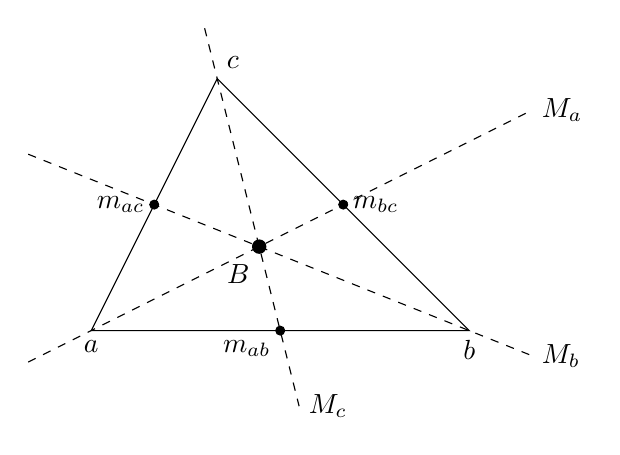
\begin{tikzpicture}[scale=0.8]
            % Coordenadas del triángulo
            \coordinate (a) at (0,0);
            \coordinate (b) at (6,0);
            \coordinate (c) at (2,4);
            \draw (a) -- (b) -- (c) -- cycle;
        
            % Etiqueta los vértices
            \node[below] at (a) {$a$};
            \node[below] at (b) {$b$};
            \node[above right] at (c) {$c$};

            % Coordenadas del baricentro
            \coordinate (B) at (8/3,4/3);
            \filldraw (B) circle (3pt) node[anchor=north east, yshift=-3pt] {$B$};

            % Coordenadas del punto medio
            \coordinate (m_AB) at (3,0);
            \filldraw (m_AB) circle (2pt) node[anchor=north east] {$m_{ab}$};
            \coordinate (m_BC) at (4,2);
            \filldraw (m_BC) circle (2pt) node[anchor=west] {$m_{bc}$};
            \coordinate (m_AC) at (1,2);
            \filldraw (m_AC) circle (2pt) node[anchor=east] {$m_{ac}$};

            % Coordenadas de inicio y fin de las medianas
            \coordinate (M_A_ini) at (-1,-0.5);
            \coordinate (M_A_fin) at (7,3.5);
            \draw[dashed] (M_A_ini) -- (M_A_fin);
            \node[right] at (M_A_fin) {$M_a$};

            \coordinate (M_B_ini) at (-1,2.8);
            \coordinate (M_B_fin) at (7,-0.4);
            \draw[dashed] (M_B_ini) -- (M_B_fin);
            \node[right] at (M_B_fin) {$M_b$};

            \coordinate (M_C_ini) at (1.8,4.8);
            \coordinate (M_C_fin) at (3.3,-1.2);
            \draw[dashed] (M_C_ini) -- (M_C_fin);
            \node[right] at (M_C_fin) {$M_c$};
        \end{tikzpicture}
        \caption{Baricentro $B$ de un triángulo $\{a,b,c\}$.}
    \end{figure}
\end{teo}
\begin{proof}
    Veamos en primer lugar que $B$ no depende de $q$:
    \begin{multline*}
        q + \frac{1}{3}\left(\vec{qa} + \vec{qb} + \vec{qc}\right) = q' + \frac{1}{3}\left(\vec{q'a} + \vec{q'b} + \vec{q'c}\right) 
        \Longleftrightarrow \\
        \Longleftrightarrow
        \vec{q'q} = \frac{1}{3}\left(a+b+c-3q'-a-b-c+3a\right)
        \Longleftrightarrow
        \vec{q'q} = \frac{1}{3}\left(-3q'+3q\right)
        \Longleftrightarrow\\ \Longleftrightarrow
        \vec{q'q} = -q'+q = \vec{q'q}
    \end{multline*}

    Veamos que $B\in M_a$. Tenemos que $M_a = a + \cc{L}\{\vec{am_{bc}}\}$. Por tanto, buscamos $\lambda\in \bb{R}$ tal que:
    \begin{equation*}
        \vec{aB} = \lambda \vec{am_{bc}}
    \end{equation*}

    De la definición de punto medio, tenemos:
    \begin{equation*}
        \vec{am_{bc}} = m_{bc} - a = q+\frac{1}{2}(\vec{qb} + \vec{qc}) -a = \vec{aq}+\frac{1}{2}(\vec{qb} + \vec{qc}) \qquad \forall q\in \cc{A}
    \end{equation*}

    De la definición de baricentro, tenemos:
    \begin{equation*}
        \vec{aB} = B-a = \vec{aq} + \frac{1}{3}\left(\vec{qa} + \vec{qb} + \vec{qc}\right)
        = \frac{2}{3}\vec{aq} + \frac{1}{3}(\vec{qb} + \vec{qc})
    \end{equation*}

    Por tanto, vemos claramente que $\vec{aB}=\frac{2}{3}\vec{am_{bc}}$. Por tanto, $B\in M_a$. Análogamente, se demuestra que $B\in M_c,M_b$, por lo que $B\in M_a\cap M_b\cap M_c$.

    Por la fórmula de las dimensiones, deducimos que $$\{B\}=M_a\cap M_b\cap M_c.$$
\end{proof}


\begin{definicion}[Mediatriz]
    Sea $\bb{E}$ un espacio euclídeo. Dado $a,b\in \bb{E}$, definimos la mediatriz del segmento $[a,b]$ como el único subespacio afín perpendicular a la recta $\langle\{ a,b\}\rangle$ que pasa por el punto medio. Es decir,
    $$L=r^\perp_{m_{ab}} = m_{ab} + \vec{r}^\perp$$
    donde $r$ es la recta que une $a,b$, es decir, $r=a+\cc{L}\{\vec{ab}\}$.
    \begin{figure}[H]
        \centering
        \begin{tikzpicture}
            \coordinate (A) at (0,0);
            \coordinate (B) at (4,0);
            \coordinate (P) at (2,2);
            
            \draw[dashed] (A) -- (B); % Dibuja el segmento AB
            
            % Mediatriz
            \path (A) -- (B) coordinate[midway] (M); % Punto medio
            \draw[-stealth] (M) -- ($(M)!1.5cm!90:(B)$); % Dibuja la mediatriz
            \draw[-stealth] (M) -- ($(M)!-1.5cm!90:(B)$); % Extiende la mediatriz hacia abajo

            \tkzMarkRightAngle[size=0.3](B,M,P)
        
            % Marcar los puntos con círculos rellenos
            \filldraw (A) circle (2pt) node[anchor=east] {$a$};
            \filldraw (B) circle (2pt) node[anchor=west] {$b$};
            \filldraw (M) circle (2pt) node[anchor=north west] {$m_{ab}$};
        \end{tikzpicture}
    \end{figure}
\end{definicion}


\begin{prop} Sea $\bb{E}$ un espacio euclídeo. Dado $a,b\in \bb{E}$, y dado $p\in \bb{E}$, se caracteriza la mediatriz de $a,b\in \bb{E}$ como:
    \begin{equation*}
        p\in r^\perp_{m_{ab}} \Longleftrightarrow d(a,p)=d(b,p)
    \end{equation*}
    \begin{figure}[H]
        \centering
        \begin{tikzpicture}
            \coordinate (A) at (0,0);
            \coordinate (B) at (4,0);
            \coordinate (P) at (2,1);
            
            \draw[dashed] (A) -- (B); % Dibuja el segmento AB

            \draw[dashed] (P) -- (A); % Dibuja el segmento AP
            \draw[dashed] (P) -- (B); % Dibuja el segmento BP
            
            % Mediatriz
            \path (A) -- (B) coordinate[midway] (M); % Punto medio
            \draw[-stealth] (M) -- ($(M)!1.5cm!90:(B)$); % Dibuja la mediatriz
            \draw[-stealth] (M) -- ($(M)!-0.5cm!90:(B)$); % Extiende la mediatriz hacia abajo

            \tkzMarkRightAngle[size=0.3](B,M,P)
        
            % Marcar los puntos con círculos rellenos
            \filldraw (A) circle (2pt) node[anchor=east] {$a$};
            \filldraw (B) circle (2pt) node[anchor=west] {$b$};
            \filldraw (M) circle (2pt) node[anchor=north west] {$m_{ab}$};

            \filldraw (P) circle (2pt) node[anchor=west] {$p$};
        \end{tikzpicture}
    \end{figure}
\end{prop}
\begin{proof}\
    \begin{description}
        \item[$\Longrightarrow)$]
        \begin{comment}
         Veamos en primer lugar que $\|\vec{m_{ab}a}\|=\|\vec{m_{ab}b}\|$:
        \begin{gather*}
            \vec{m_{ab}a} = a-m_{ab}=a-a-\frac{1}{2}\vec{ab} = -\frac{1}{2}\vec{ab} \Longrightarrow ||\vec{m_{ab}a}|| = \frac{1}{2}\|\vec{ab}\|\\
            \vec{m_{ab}b} = b-m_{ab}=b-a-\frac{1}{2}\vec{ab} = \vec{ab}-\frac{1}{2}\vec{ab} = \frac{1}{2}\vec{ab} \Longrightarrow ||\vec{m_{ab}b}|| = \frac{1}{2}\|\vec{ab}\|
        \end{gather*}
        
        
        Veamos ahora que $\vec{pm_{ab}}\perp \vec{m_{ab}a}$. Para ello, vemos que $\vec{m_{ab}a}\in \vec{r}$:
        \begin{equation*}
            \vec{m_{ab}a}=a-m_{ab}=a-a-\frac{1}{2}\vec{ab}=-\frac{1}{2}\vec{ab}\in \cc{L}\{\vec{ab}\}
        \end{equation*}
        Análogamente, tenemos que $\vec{m_{ab}b}\in \vec{r}$. Además, tenemos que $p,m_{ab}\in r_{m_{ab}}^\perp$, por lo que $\vec{m_{ab}p}\in \vec{r}^\perp$. Por tanto, por definición de subespacio ortogonal, tenemos que $\vec{m_{ab}p}\perp \vec{m_{ab}a},\vec{m_{ab}b}$.

        Por tanto, por el Teorema de Pitágoras, tenemos que:
        \begin{equation*}
            \|\vec{pa}\|^2 = \|\vec{m_{ab}p}\|^2 + \|\vec{m_{ab}a}\|^2 \AstIg \|\vec{m_{ab}p}\|^2 + \|\vec{m_{ab}b}\|^2 = \|\vec{pb}\|^2
        \end{equation*}
        donde en $(\ast)$ he aplicado que $\|\vec{m_{ab}a}\|=\|\vec{m_{ab}b}\|$. Por tanto, tenemos que $\|\vec{pa}\|=\|\vec{pb}\|$, por lo que:
        \begin{equation*}
            d(a,p)=\|a-p\| = \|\vec{pa}\|=\|\vec{pb}\| = \|b-p\| = d(b,p)
        \end{equation*}
        \end{comment}

        Si $p\in r_{m_{ab}}^\perp$, entonces $\vec{m_{ab}p}\perp \vec{ab}$. Los triángulos $\{p,a,m_{ab}\}$ y $\{p,b,m_{ab}\}$ son rectángulos. Por tanto, por el Teorema de Pitágoras,
        \begin{equation*}
            d^2(a,p) = d^2(a,m_{ab}) + d^2(p,m_{ab}) = d^2(b,m_{ab}) + d^2(p,m_{ab})
            = d^2(b,p)
        \end{equation*}
        Por tanto, $d(a,p)=d(b,p)$.
        
        \item[$\Longleftarrow)$] Supongamos que $p\notin r_{m_{ab}}^\perp$, y lleguemos a una contradicción.
        
        Como $p\notin r_{m_{ab}}^\perp$, tenemos que $\vec{m_{ab}p}\notin \vec{r}^\perp$. Por tanto, $\exists v\in \cc{L}\{\vec{ab}\}$ tal que $\langle v,\vec{m_{ab}p}\rangle\neq 0$. Como $v\in \cc{L}\{\vec{ab}\}$, tenemos que $v=k\cdot \frac{1}{2}\vec{ab}$ para cierto $k\in \bb{R}^\ast$. Por tanto,
        \begin{equation*}
            0\neq \langle v,\vec{m_{ab}p}\rangle = \left\langle k\cdot \frac{1}{2}\vec{ab},\vec{m_{ab}p}\right\rangle
            = k \left\langle \frac{1}{2}\vec{ab},\vec{m_{ab}p}\right\rangle
            = k \left\langle \vec{m_{ab}b},\vec{m_{ab}p}\right\rangle
            = -k \left\langle \vec{m_{ab}a},\vec{m_{ab}p}\right\rangle
        \end{equation*}

        Por tanto, tenemos que $\vec{m_{ab}p}\not \perp \vec{m_{ab}a},\vec{m_{ab}b}$. Por el Teorema de Pitágoras, tenemos que:
        \begin{equation*}
            \|\vec{pa}\|^2 \neq \|\vec{m_{ab}p}\|^2 + \|\vec{m_{ab}a}\|^2 \AstIg \|\vec{m_{ab}p}\|^2 + \|\vec{m_{ab}b}\|^2 \neq \|\vec{pb}\|^2
        \end{equation*}
        donde en $(\ast)$ he aplicado que $\|\vec{m_{ab}a}\|=\|\vec{m_{ab}b}\|$. Por tanto, tenemos que $\|\vec{pa}\|\neq\|\vec{pb}\|$, por lo que:
        \begin{equation*}
            d(a,p)=\|a-p\| = \|\vec{pa}\|\neq \|\vec{pb}\| = \|b-p\| = d(b,p)
        \end{equation*}
        llegando entonces a una contradicción. Por tanto, $p\in r_{m_{ab}}^\perp$.
    \end{description}
\end{proof}

\begin{teo}[Circuncentro]
    Sea $\bb{E}$ un espacio euclídeo. Dado un triángulo $\{a,b,c\}\subset~\bb{E}$. Notemos $R_a$ a la mediatriz del segmento $[b,c]$, y análogamente a $R_b,R_c$.
    
    Entonces, las tres mediatrices se cortan en un único punto, $C\in \bb{E}$, llamado circuncentro.
    \begin{equation*}
        \{C\}=R_a\cap R_b\cap R_c
    \end{equation*}

    \begin{figure}[H]
        \centering
        \begin{tikzpicture}[scale=0.8]
            % Coordenadas del triángulo
            \coordinate (a) at (0,0);
            \coordinate (b) at (6,0);
            \coordinate (c) at (2,4);
            \draw (a) -- (b) -- (c) -- cycle;
        
            % Etiqueta los vértices
            \node[below] at (a) {$a$};
            \node[right] at (b) {$b$};
            \node[above] at (c) {$c$};

            % Coordenadas del circuncentro
            \coordinate (C) at (3,1);
            \filldraw (C) circle (3pt) node[anchor=west, , xshift=10pt] {$C$};

            % Coordenadas del punto medio
            \coordinate (m_AB) at (3,0);
            \filldraw (m_AB) circle (2pt) node[anchor=north west] {$m_{ab}$};
            \coordinate (m_BC) at (4,2);
            \filldraw (m_BC) circle (2pt) node[anchor=west] {$m_{bc}$};
            \coordinate (m_AC) at (1,2);
            \filldraw (m_AC) circle (2pt) node[anchor=east] {$m_{ac}$};

            % Coordenadas de inicio y fin de las mediatrices
            \coordinate (R_A_ini) at (1,-1);
            \coordinate (R_A_fin) at (6,4);
            \draw[dashed] (R_A_ini) -- (R_A_fin);
            \node[right] at (R_A_fin) {$R_a$};

            \coordinate (R_B_ini) at (-1,3);
            \coordinate (R_B_fin) at (7,-1);
            \draw[dashed] (R_B_ini) -- (R_B_fin);
            \node[right] at (R_B_fin) {$R_b$};

            \coordinate (R_C_ini) at (3, -1);
            \coordinate (R_C_fin) at (3,5);
            \draw[dashed] (R_C_ini) -- (R_C_fin);
            \node[right] at (R_C_fin) {$R_c$};

            % Coordenadas de los puntos de corte para marcar los ángulos
            \coordinate (T_a) at (4,2);
            \coordinate (T_b) at (1,2);
            \coordinate (T_c) at (3,0);
            \tkzMarkRightAngle[size=0.3](a,T_c,C);
            \tkzMarkRightAngle[size=0.3](b,T_a,C);
            \tkzMarkRightAngle[size=0.3](c,T_b,C);
        \end{tikzpicture}
        \caption{Cincuncentro $C$ de un triángulo $\{a,b,c\}$.}
    \end{figure}
\end{teo}
\begin{proof}
    Veamos en primer lugar que $R_a \cancel{\|} R_b$. Si fuesen paralelas, entones $\vec{R_a}=\vec{R_b}$ Es decir, ${\cc{L}\left\{\vec{bc}\right\}^\perp} = {\cc{L}\{\vec{ac}\}^\perp}$. Por tanto, tendríamos que ambas rectas vectoriales serían iguales, por lo que sus vectores directores serían linealmente dependientes, algo que no es posible ya que los tres vértices de un triángulo son afínmente independientes. Por tanto, las mediatrices no son paralelas dos a dos.

    Por tanto, $\exists C\in R_a\cap R_b$. Es decir, $C$ es un único punto y como $C\in R_a$, entonces $d(C,b)=d(C,c)$. Además, como $C\in R_b$, entonces $d(C,a)=d(C,c)$. Por tanto, el punto es equidistante de los tres vértices. Como $d(C,a)=d(C,c)=d(C,b)$, tenemos que $C\in R_c$. Por tanto,
    \begin{equation*}
        C\in R_a\cap R_b\cap R_c
    \end{equation*}

    Por la fórmula de las dimensiones, deducimos que $$\{C\}=R_a\cap R_b\cap R_c.$$
\end{proof}
Notemos que el nombre del circuncentro de sebe a que es el centro de una circunferencia que pasa por $a,b$ y $c$.


\begin{definicion}[Altura]
    Sea $\bb{E}$ un espacio euclídeo. Dado un triángulo $\{a,b,c\}\subset~\bb{E}$, se define la altura $H_a$ del vértice $a$ como la recta que pasa por $a$ y es ortogonal al lado opuesto $[b,c]$:
    \begin{equation*}
        H_a = a + \cc{L}\left\{\vec{bc}\right\}^\perp
    \end{equation*}

    Análogamente se definen las alturas asociadas a los vértices $b$ y $c$.
\end{definicion}

\begin{teo}[Ortocentro]
    Sea $\bb{E}$ un espacio euclídeo. Dado un triángulo $\{a,b,c\}\subset~\bb{E}$, existe un único punto $O\in \bb{E}$ llamado ortocentro tal que:
    \begin{equation*}
        \{O\} = H_a\cap H_b \cap H_c
    \end{equation*}
    \begin{figure}[H]
        \centering
        \begin{tikzpicture}[scale=0.8]
            % Coordenadas del triángulo
            \coordinate (a) at (0,0);
            \coordinate (b) at (6,0);
            \coordinate (c) at (2,4);
            \draw (a) -- (b) -- (c) -- cycle;
        
            % Etiqueta los vértices
            \node[left] at (a) {$a$};
            \node[below] at (b) {$b$};
            \node[left] at (c) {$c$};

            % Coordenadas del ortocentro
            \coordinate (O) at (2,2);
            \filldraw (O) circle (3pt) node[anchor=north west, yshift=-4pt] {$O$};

            % Coordenadas de inicio y fin de las alturas
            \coordinate (H_A_ini) at (-1,-1);
            \coordinate (H_A_fin) at (5,5);
            \draw[dashed] (H_A_ini) -- (H_A_fin);
            \node[right] at (H_A_fin) {$H_a$};

            \coordinate (H_B_ini) at (-1,3.5);
            \coordinate (H_B_fin) at (7,-0.5);
            \draw[dashed] (H_B_ini) -- (H_B_fin);
            \node[left] at (H_B_ini) {$H_b$};

            \coordinate (H_C_ini) at (2, -1);
            \coordinate (H_C_fin) at (2,5);
            \draw[dashed] (H_C_ini) -- (H_C_fin);
            \node[right] at (H_C_fin) {$H_c$};

            % Coordenadas de los puntos de corte para marcar los ángulos
            \coordinate (T_a) at (3,3);
            \coordinate (T_b) at (1.2,2.4);
            \coordinate (T_c) at (2,0);
            \tkzMarkRightAngle[size=0.3](b,T_c,O);
            \tkzMarkRightAngle[size=0.3](b,T_a,O);
            \tkzMarkRightAngle[size=0.3](a,T_b,O);
        \end{tikzpicture}
        \caption{Ortocentro $O$ de un triángulo $\{a,b,c\}$.}
    \end{figure}
\end{teo}
\begin{proof}
    Veamos en primer lugar que $H_a \cancel{\|} H_b$. Si fuesen paralelas, entones ${\cc{L}\left\{\vec{bc}\right\}^\perp} = {\cc{L}\{\vec{ac}\}^\perp}$. Por tanto, tendríamos que ambas rectas vectoriales serían iguales, por lo que sus vectores directores serían linealmente dependientes, algo que no es posible ya que los tres vértices de un triángulo son afínmente independientes. Por tanto, las alturas no son paralelas dos a dos.

    Como $H_a$ y $H_b$ son secantes, entonces se cortan en un punto $O\in \bb{E}$:
    \begin{equation*}
        O\in H_a\cap H_b
    \end{equation*}

    Veamos ahora que $O\in H_c$. Para ello, vemos que $\vec{Oc}\perp \vec{ab}$:
    \begin{equation*}
        \begin{split}
            \langle \vec{Oc},\vec{ab}\rangle &=
             \langle \vec{Oa} + \vec{ac},\vec{aO}+\vec{Ob}\rangle
             =
             \langle \vec{Oa},\vec{aO}+\vec{Ob}\rangle + \langle\vec{ac},\vec{aO}\rangle + \langle\vec{ac},\vec{Ob}\rangle =\\&
             =
             \langle \vec{Oa},\vec{aO}+\vec{Ob}\rangle -\langle\vec{Oa},\vec{ac}\rangle + \langle\vec{ac},\vec{Ob}\rangle
              =
             \langle \vec{Oa},\vec{aO}+\vec{Ob}-\vec{ac}\rangle + \langle\vec{ac},\vec{Ob}\rangle =\\&
             =
             \langle \vec{Oa},\vec{ca} + \vec{aO}+\vec{Ob}\rangle + \langle\vec{ac},\vec{Ob}\rangle
             =
             \langle \vec{Oa},\vec{cb}\rangle + \langle\vec{ac},\vec{Ob}\rangle = 0
        \end{split}
    \end{equation*}
    donde he usado la igualdad triangular, las propiedades de la métrica $\langle,\rangle$ y que $\langle \vec{Oa},\vec{cb}\rangle = \langle\vec{ac},\vec{Ob}\rangle = 0$ por ser $O\in H_a\cap H_b$.

    Por tanto, $O\in H_a\cap H_b\cap H_c$. Por la fórmula de las dimensiones, deducimos que $$\{O\}=H_a\cap H_b\cap H_c.$$
\end{proof}


\begin{teo}[De Euler]\label{teo:euler}
    Sea $\bb{E}$ un espacio euclídeo. Dado un triángulo $\{a,b,c\}\subset~\bb{E}$, el baricentro $B$, el circuncentro $C$ y el ortocentro $O$ están alineados.


    Si $\{B,C,O\}$ contiene al menos dos puntos distintos, la recta pasando por $B,C$ y $O$ se denomina \ul{Recta de Euler}.
    \begin{figure}[H]
        \centering
        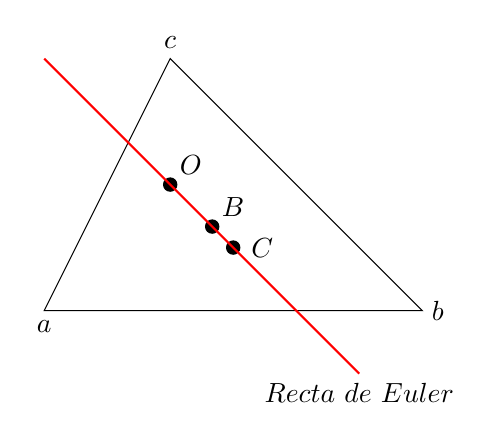
\begin{tikzpicture}[scale=0.8]
            % Coordenadas del triángulo
            \coordinate (a) at (0,0);
            \coordinate (b) at (6,0);
            \coordinate (c) at (2,4);
            \draw (a) -- (b) -- (c) -- cycle;
        
            % Etiqueta los vértices
            \node[below] at (a) {$a$};
            \node[right] at (b) {$b$};
            \node[above] at (c) {$c$};

            % Coordenadas del circuncentro
            \coordinate (C) at (3,1);
            \filldraw (C) circle (3pt) node[anchor=west, xshift=3pt] {$C$};

            \coordinate (O) at (2,2);
            \filldraw (O) circle (3pt) node[anchor=south west] {$O$};

            \coordinate (B) at (8/3,4/3);
            \filldraw (B) circle (3pt) node[anchor=south west] {$B$};

            % Coordenadas de inicio y fin de las mediatrices
            \coordinate (E_ini) at (0,4);
            \coordinate (E_fin) at (5,-1);
            \draw[thick, red] (E_ini) -- (E_fin);
            \node[below] at (E_fin) {$Recta$ $de$ $Euler$};
        \end{tikzpicture}
    \end{figure}
\end{teo}
\begin{proof}
    Consideramos la homotecia de razón $k=-\frac{1}{2}$ y centro el baricentro $B$. Veamos que $H_{B,-\nicefrac{1}{2}}$ lleva cada vértice en el punto medio del segmento opuesto:
    \begin{equation*}\begin{split}
        H_{B,-\nicefrac{1}{2}}(a) &= B -\frac{1}{2}\vec{Ba} = B +\frac{1}{2}\vec{aB}
        = \left(a + \frac{1}{3}\left(\vec{ab} + \vec{ac}\right)\right) + \frac{1}{2}\left[\left(\cancel{a} + \frac{1}{3}\left(\vec{ab} + \vec{ac}\right)\right)-\cancel{a}\right]=\\
        &= \left(a + \frac{1}{3}\left(\vec{ab} + \vec{ac}\right)\right) + \frac{1}{6}\left(\vec{ab} + \vec{ac}\right)
        = a + \frac{1}{2}\left(\vec{ab} + \vec{ac}\right) = m_{bc}
    \end{split}\end{equation*}
    \begin{figure}[H]
        \centering
        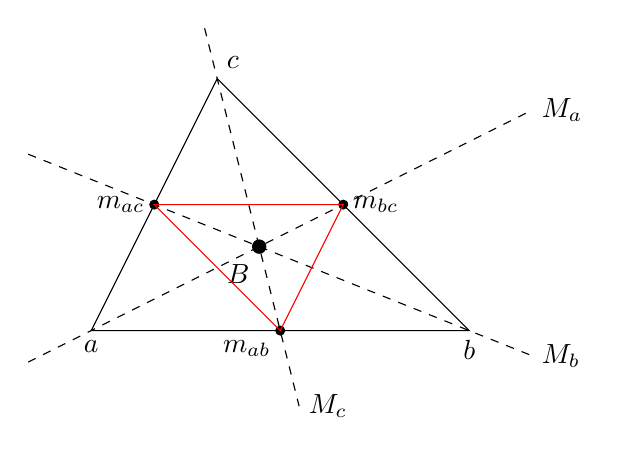
\begin{tikzpicture}[scale=0.8]
            % Coordenadas del triángulo
            \coordinate (a) at (0,0);
            \coordinate (b) at (6,0);
            \coordinate (c) at (2,4);
            \draw (a) -- (b) -- (c) -- cycle;
        
            % Etiqueta los vértices
            \node[below] at (a) {$a$};
            \node[below] at (b) {$b$};
            \node[above right] at (c) {$c$};
    
            % Coordenadas del baricentro
            \coordinate (B) at (8/3,4/3);
            \filldraw (B) circle (3pt) node[anchor=north east, yshift=-3pt] {$B$};
    
            % Coordenadas del punto medio
            \coordinate (m_AB) at (3,0);
            \filldraw (m_AB) circle (2pt) node[anchor=north east] {$m_{ab}$};
            \coordinate (m_BC) at (4,2);
            \filldraw (m_BC) circle (2pt) node[anchor=west] {$m_{bc}$};
            \coordinate (m_AC) at (1,2);
            \filldraw (m_AC) circle (2pt) node[anchor=east] {$m_{ac}$};
    
            % Coordenadas de inicio y fin de las medianas
            \coordinate (M_A_ini) at (-1,-0.5);
            \coordinate (M_A_fin) at (7,3.5);
            \draw[dashed] (M_A_ini) -- (M_A_fin);
            \node[right] at (M_A_fin) {$M_a$};
    
            \coordinate (M_B_ini) at (-1,2.8);
            \coordinate (M_B_fin) at (7,-0.4);
            \draw[dashed] (M_B_ini) -- (M_B_fin);
            \node[right] at (M_B_fin) {$M_b$};
    
            \coordinate (M_C_ini) at (1.8,4.8);
            \coordinate (M_C_fin) at (3.3,-1.2);
            \draw[dashed] (M_C_ini) -- (M_C_fin);
            \node[right] at (M_C_fin) {$M_c$};
    
            % triángulo interior
            \draw[red] (m_AB) -- (m_AC) -- (m_BC) -- cycle;
        \end{tikzpicture}
        \caption{\centering Baricentro $B$ de un triángulo $\{a,b,c\}$, junto con el triángulo formado por $H_{B,-\nicefrac{1}{2}}$.}
    \end{figure}
    Análogamente se demuestra para $b,c$, por lo que se tiene que $H_{B,-\nicefrac{1}{2}}$ lleva cada vértice en el punto medio del segmento opuesto. Veamos ahora que $h$ lleva las alturas de $\{a,b,c\}$ en las mediatrices de $\{a,b,c\}$:
    \begin{multline*}
        H_{B,-\nicefrac{1}{2}}(H_a) = H_{B,-\nicefrac{1}{2}}\left(a + \cc{L}\left\{\vec{bc}\right\}^\perp\right)
        = H_{B,-\nicefrac{1}{2}}(a) -\frac{1}{2}Id_{\vec{\bb{E}}}\left(\cc{L}\left\{\vec{bc}\right\}^\perp\right) =\\= m_{bc} + \cc{L}\left\{\vec{bc}\right\}^\perp= R_a
    \end{multline*}
    
    Análogamente, se demuestra para $H_b, H_c$, por lo que:
    \begin{equation*}
        H_{B,-\nicefrac{1}{2}}(O) = H_{B,-\nicefrac{1}{2}}(H_a) \cap H_{B,-\nicefrac{1}{2}}(H_b) = H_{B,-\nicefrac{1}{2}}(H_c) = R_a\cap R_b \cap R_c = C
    \end{equation*}
    
    No obstante, se tiene que un punto, su imagen mediante una homotecia de centro $o$, y el mismo centro $o$ están alineados. Por tanto, $O, C=H_{B,-\nicefrac{1}{2}}(O)$ y $B$ están alineados, como queríamos demostrar.
\end{proof}

\subsection{Incentro}

En este apartado, introducimos el cuarto punto notable del triángulo, el incentro. Separamos este punto del resto por no estar este contenido, de forma general, en la recta de Euler.
Para definirlo, hemos de introducir el concepto de bisectriz, seguramente conocido por el lector.
\begin{definicion}[Bisectriz de dos rectas secantes]
    Sea $\bb{E}$ un espacio euclídeo. Sean dos rectas secantes $R_1,R_2\subset \bb{E}$, con $R_1=p + \cc{L}\{v_1\}$ y $R_2=p + \cc{L}\{v_2\}$.
    Consideramos los vectores $u_a,u_b\in \vec{\bb{E}}$ tales que:
    \begin{equation*}
        u_a := \frac{v_1}{\|v_1\|} + \frac{v_2}{\|v_2\|} \qquad u_b := \frac{v_1}{\|v_1\|} - \frac{v_2}{\|v_2\|}
    \end{equation*}

    Entonces, las dos bisectrices de $R_1$ y $R_2$ son las rectas $B_a,B_b\subset \bb{E}$ dadas por:
    \begin{equation*}
        B_a = p + \cc{L}\{u_a\} \qquad B_b = p + \cc{L}\{u_b\}
    \end{equation*}

    \begin{figure}[H]
        \centering
        \begin{tikzpicture}[scale=0.6]
            % Define los puntos de las rectas
            \coordinate (r1_ini) at (-4,-2);
            \coordinate (r1_fin) at (4,2);
            \coordinate (r2_ini) at (-4,2);
            \coordinate (r2_fin) at (4,-2);

            \coordinate (O) at (0,0);
            \coordinate (v_1) at (2,1);
            \coordinate (v_2) at (2,-1);

            \coordinate (u_a) at (4,0);
            \coordinate (u_b) at (0,2);

            % Define las bisectrices
            \coordinate (B_a_ini) at (-6,0);
            \coordinate (B_a_fin) at (6,0);
            \coordinate (B_b_ini) at (0,-3);
            \coordinate (B_b_fin) at (0,3);
        
            % Dibuja las rectas
            \draw[dashed] (r1_ini) -- (r1_fin) node[right] {$R_1$};
            \draw[dashed] (r2_ini) -- (r2_fin) node[right] {$R_2$};

            % Dibuja los vectores directores
            \draw[-stealth, teal] (O) -- node[above]{$v_1$} (v_1);
            \draw[-stealth, teal] (O) -- node[below]{$v_2$} (v_2);

            % Dibuja las bisectrices
            \draw[] (B_a_ini) -- (B_a_fin) node[right] {$B_a$};
            \draw[] (B_b_ini) -- (B_b_fin) node[right] {$B_b$};

            % Dibuja los vectores directores de las bisectrices
            \draw[-stealth, blue] (O) -- (u_a) node[above]{$u_a$};
            \draw[-stealth, red] (O) -- (u_b) node[left]{$u_b$};

            %\tkzMarkAngle[size=0.5](v_2,O,v_1);
            %\tkzLabelAngle[pos=0.8](v_2,O,v_1){$\alpha$};

            % Punto de intersección
            \filldraw[black] (O) circle (2pt) node[above left] {$p$};
        \end{tikzpicture}
        \caption{Bisectrices de las rectas $R_1$ y $R_2$.}
    \end{figure}
\end{definicion}

\begin{lema}
    Sea $\bb{E}$ un espacio euclídeo. Sean $R_1,R_2\subset \bb{E}$ dos rectas secantes, y sean $B_a,B_b$ sus bisectrices. Entonces:
    \begin{equation*}
        B_a \perp B_b
    \end{equation*}
\end{lema}
\begin{proof}
    Tenemos que:
    \begin{align*}
        \langle u_a,u_b\rangle
        &= \left\langle \frac{v_1}{\|v_1\|} + \frac{v_2}{\|v_2\|}, \frac{v_1}{\|v_1\|} - \frac{v_2}{\|v_2\|}\right\rangle = \\
        &= \frac{\|v_1\|^2}{\|v_1\|^2} - \cancel{\frac{\langle v_1, v_2\rangle}{\|v_1\|~\|v_2\|}} + \cancel{\frac{\langle v_2, v_1\rangle}{\|v_1\|~\|v_2\|}} - \frac{\|v_2\|^2}{\|v_2\|^2}
        =1-1= 0
    \end{align*}
\end{proof}

\begin{prop} \label{prop:BisectrizDivideAngulo}
    Sea $\bb{E}$ un espacio euclídeo. Sean $R_1,R_2\subset \bb{E}$ dos rectas secantes y sea $B\subset \bb{E}$ una recta. Entonces:
    \begin{equation*}
        B \text{ es una bisectriz de $R_1$ y $R_2$} \sii \measuredangle(R_1,B) = \measuredangle(R_2,B)
    \end{equation*}
\end{prop}
\begin{comment}
    % // TODO: Demostración Bisectriz divide ángulo en dos ángulos iguales
\begin{proof}
    Sea $p\in R_1\cap R_2$. Consideramos $u_a,u_b\in \vec{\bb{E}}$ tales que:
    \begin{equation*}
        u_a := \frac{v_1}{\|v_1\|} + \frac{v_2}{\|v_2\|} \qquad u_b := \frac{v_1}{\|v_1\|} - \frac{v_2}{\|v_2\|}
    \end{equation*}
    donde $v_1,v_2$ son los vectores directores \ul{unitarios} de $R_1$ y $R_2$ respectivamente. Sean las bisectrices $B_a=p+\cc{L}\{u_a\}$ y $B_b=p+\cc{L}\{u_b\}$.
    Tenemos que:
    \begin{equation*}
        \langle u_a, v_1\rangle
        = \left\langle \frac{v_1}{\|v_1\|} + \frac{v_2}{\|v_2\|}, v_1\right\rangle
        = \frac{1}{\|v_1\|}\langle v_1,v_1\rangle + \frac{1}{\|v_2\|}\langle v_2,v_1\rangle = \|v_1\| + \frac{1}{\|v_2\|} \langle v_2,v_1\rangle
    \end{equation*}
    \begin{equation*}
        \langle u_a, v_2\rangle
        = \left\langle \frac{v_1}{\|v_1\|} + \frac{v_2}{\|v_2\|}, v_2\right\rangle
        = \frac{1}{\|v_1\|}\langle v_1,v_2\rangle + \frac{1}{\|v_2\|}\langle v_2,v_2\rangle = \frac{1}{\|v_1\|} \langle v_1,v_2\rangle + \|v_2\|
    \end{equation*}
    \begin{equation*}
        \|v_1\|\cdot \left\|u_a\right\| = \|v_1\|\cdot \left\| \frac{v_1}{\|v_1\|} + \frac{v_2}{\|v_2\|}\right\|
        = \left\|v_1 + \frac{\|v_1\|}{\|v_2\|}\cdot v_2\right\|
    \end{equation*}
    \begin{equation*}
        \|v_2\|\cdot \left\|u_a\right\| = \|v_2\|\cdot \left\| \frac{v_1}{\|v_1\|} + \frac{v_2}{\|v_2\|}\right\|
        = \left\|\frac{\|v_2\|}{\|v_1\|}\cdot v_1 + v_2\right\|
    \end{equation*}

    Usando que $\langle v_1,v_2\rangle = \langle v_2,v_1\rangle$ y que, por la elección de $v_1,v_2$ con $\|v_1\|=\|v_2\|=1$, tenemos que:
    \begin{equation*}
        \cos \measuredangle(v_1,u_a) = \cos \measuredangle(v_2,u_a) 
    \end{equation*}


    Para comprobar que el ángulo es el mismo, basta comprobar que el ángulo entre los vectores directores de $R_1$ y $B_a$ es el mismo que el ángulo entre los vectores directores de $R_2$ y $B_a$. Es decir, basta comprobar que:
\end{proof}
\end{comment}

\begin{prop}\label{prop:BisectrizEquidistante}
    Sea $\bb{E}$ un espacio euclídeo. Sean $R_1,R_2\subset \bb{E}$ dos rectas secantes, y sea $B$ una de sus bisectrices. Entonces, dado $q\in \bb{E}$, se tiene que:
    \begin{equation*}
        q\in B \sii d(q,R_1)=d(q,R_2)
    \end{equation*}
    % // TODO: Demostración de que la bisectriz es el lugar geométrico de los puntos equidistantes a las rectas
\end{prop}

\begin{observacion}
    Aunque dos rectas tengan dos bisectrices, se suele hablar de \ul{la} bisectriz de dos rectas. Al igual forma que se vio que dos rectas forman
    dos ángulos $\alpha,\beta$ tal que $\alpha+\beta=\pi$, y se definía el ángulo entre dos rectas como el menor de los dos ángulos, cuando se
    habla de la bisectriz de dos rectas, se refiere a la bisectriz del ángulo menor.\\
\end{observacion}

Aunque las bisectrices se definan para las rectas, es común extender el concepto a otros elementos geométricos, como hablar de \emph{bisectriz de un ángulo},
\emph{bisectriz en un vértice}, etc. Ejemplo de esto es la siguiente definición:
\begin{definicion}
    Sea $\bb{E}$ un espacio euclídeo. Dados tres puntos $a,b,c\in \bb{E}$ no alineados, se define la bisectriz del ángulo $\measuredangle(bac)$
    en el vértice $a$ como la bisectriz de las rectas $R_b=a+\cc{L}\{\vec{ab}\}$ y $R_c=a+\cc{L}\{\vec{ac}\}$.
\end{definicion}


Una vez introducido el concepto de bisectriz de forma general, concretamos para el caso de un triángulo, que es el caso que nos interesa. Al igual que
en el caso del resto de los puntos notables, el incentro se define como el punto de corte de las bisectrices de los ángulos de un triángulo.
\begin{teo}[Incentro]\label{teo:incentro}
    Sea $\bb{E}$ un espacio euclídeo. Dado un triángulo $\{a,b,c\}\subset~\bb{E}$, notamos por $I_a,I_b,I_c$ a las bisectrices de los ángulos
    $\measuredangle(bac),\measuredangle(abc),\measuredangle(cba)$ en los vértices $a,b,c$ respectivamente. Es decir:
    \begin{gather*}
        I_a = a + \cc{L}\left\{\frac{\vec{ab}}{\left\|\vec{ab}\right\|} + \frac{\vec{ac}}{\left\|\vec{ac}\right\|}\right\} \qquad
        I_b = b + \cc{L}\left\{\frac{\vec{ba}}{\left\|\vec{ba}\right\|} + \frac{\vec{bc}}{\left\|\vec{bc}\right\|}\right\} \\
        I_c = c + \cc{L}\left\{\frac{\vec{ca}}{\left\|\vec{ca}\right\|} + \frac{\vec{cb}}{\left\|\vec{cb}\right\|}\right\}
    \end{gather*}
    
    Entonces, existe un único punto $I\in \bb{E}$ llamado incentro tal que:
    \begin{equation*}
        \{I\} = I_a\cap I_b \cap I_c
    \end{equation*}

    \begin{figure}[H]
        \centering
        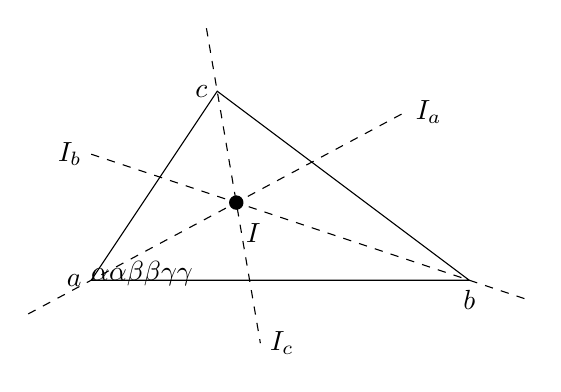
\begin{tikzpicture}[scale=0.8]

            % Coordenadas del triángulo
            \coordinate (a) at (0,0);
            \coordinate (b) at (6,0);
            \coordinate (c) at (2,3);
            \draw (a) -- (b) -- (c) -- cycle;
        
            % Etiqueta los vértices
            \node[left] at (a) {$a$};
            \node[below] at (b) {$b$};
            \node[left] at (c) {$c$};

            % Coordenadas del incentro
            \coordinate (I) at (2.30277, 1.232408);
            \filldraw (I) circle (3pt) node[anchor=north west, yshift=-4pt] {$I$};

            % Coordenadas de inicio y fin de las alturas
            \coordinate (I_A_ini) at (-1,-0.53517);
            \coordinate (I_A_fin) at (5,2.676);
            \draw[dashed] (I_A_ini) -- (I_A_fin);
            \node[right] at (I_A_fin) {$I_a$};

            \coordinate (I_B_ini) at (0,2);
            \coordinate (I_B_fin) at (7, -1/3);
            \draw[dashed] (I_B_ini) -- (I_B_fin);
            \node[left] at (I_B_ini) {$I_b$};

            \coordinate (I_C_ini) at (1.82872, 4);
            \coordinate (I_C_fin) at (2.685162, -1);
            \draw[dashed] (I_C_ini) -- (I_C_fin);
            \node[right] at (I_C_fin) {$I_c$};

            % Coordenadas de los puntos de corte para marcar los ángulos
            \tkzMarkAngle[size=1 , red](I,a,c);
            \tkzLabelAngle[pos=1.4, red](I,a,c){$\alpha$};
            \tkzMarkAngle[size=0.8, red](b,a,I);
            \tkzLabelAngle[pos=1.1, red](b,a,I){$\alpha$};

            \tkzMarkAngle[size=1, blue](I,b,a);
            \tkzLabelAngle[pos=1.3, blue](I,b,a){$\beta$};
            \tkzMarkAngle[size=1.3, blue](c,b,I);
            \tkzLabelAngle[pos=1.6, blue](c,b,I){$\beta$};

            \tkzMarkAngle[size=0.5, teal](I,c,b);
            \tkzLabelAngle[pos=0.8, teal](I,c,b){$\gamma$};
            \tkzMarkAngle[size=0.8, teal](a,c,I);
            \tkzLabelAngle[pos=1.1, teal](a,c,I){$\gamma$};
            
        \end{tikzpicture}
        \caption{Incentro $I$ de un triángulo $\{a,b,c\}$.}
    \end{figure}
\end{teo}
\begin{proof}
    Veamos en primer lugar que $I_a$, $I_b$ no son paralelas. Si lo fuesen,
    entones tendríamos que $\exists \lm \in \bb{R}$ tal que:
    \begin{equation*}
        \frac{\vec{ab}}{\left\|\vec{ab}\right\|} + \frac{\vec{ac}}{\left\|\vec{ac}\right\|} = \lm 
        \cdot \left(\frac{\vec{ba}}{\left\|\vec{ba}\right\|} + \frac{\vec{bc}}{\left\|\vec{bc}\right\|}\right)
        \Longrightarrow \vec{ab}\left(\frac{1}{\left\|\vec{ab}\right\|} + \lm\right)
        + \frac{\vec{ac}}{\left\|\vec{ac}\right\|} = \lm \cdot \frac{\vec{bc}}{\left\|\vec{bc}\right\|}
    \end{equation*}

    Por la igualdad triangular, tenemos que: $\vec{bc} = -\vec{ab} + \vec{ac}$. Por tanto,
    \begin{equation*}
        \vec{ab}\left(\frac{1}{\left\|\vec{ab}\right\|} + \lm + \frac{\lm}{\left\|\vec{bc}\right\|}\right)
        + \frac{\vec{ac}}{\left\|\vec{ac}\right\|}\left(1 - \frac{\lm}{\left\|\vec{bc}\right\|}\right) = 0
    \end{equation*}

    Como $\left\{\vec{ab},\vec{ac}\right\}$ son linealmente independientes, entonces:
    \begin{equation*}
        1 - \frac{\lm}{\left\|\vec{bc}\right\|} = 0 = \frac{1}{\left\|\vec{ab}\right\|} + \lm + \frac{\lm}{\left\|\vec{bc}\right\|}
    \end{equation*}

    De la igualdad de la izquierda, obtenemos que $\lm = \left\|\vec{bc}\right\|$. Sustituyendo en la igualdad de la derecha, tenemos que:
    \begin{equation*}
        \frac{1}{\left\|\vec{ab}\right\|} + \left\|\vec{bc}\right\| + 1 = 0
    \end{equation*}
    No obstante, esto es imposible, ya que es una suma de términos positivos. Por tanto, $I_a$ y $I_b$ no son paralelas.
    Como $I_a$ y $I_b$ son secantes, entonces se cortan en un punto $I\in \bb{E}$:
    \begin{equation*}
        I\in I_a\cap I_b
    \end{equation*}
    
    Veamos ahora que $I\in I_c$. Como $I\in I_a$, entonces $\d(I, R_{ab})=\d(I, R_{ac})$.
    Como $I\in I_b$, entonces $\d(I, R_{bc})=\d(I, R_{ab})$. Por tanto, tenemos que:
    \begin{equation*}
        \d(I, R_{bc})=\d(I, R_{ab})=\d(I, R_{ac}) \Longrightarrow d(I, R_{bc})=d(I, R_{ac}) \Longrightarrow I\in I_c
    \end{equation*}

    Por tanto, tenemos que $I\in I_a\cap I_b\cap I_c$. Por la fórmula de las dimensiones, tenemos que:
    \begin{equation*}
        \{I\} = I_a\cap I_b \cap I_c
    \end{equation*}
    Por tanto, queda también así demostrada la unicidad de $I$.

    \begin{comment}
    Para ello, veremos que $\vec{cI}\in \cc{L}\left\{\frac{\vec{ca}}{\left\|\vec{ca}\right\|} + \frac{\vec{cb}}{\left\|\vec{cb}\right\|}\right\}$.
    Por la igualdad triangular y como $I\in I_a$, entonces $\exists \lm_a\in \bb{R}$ tal que:
    \begin{align*}
        \vec{cI} &= \vec{ca} + \vec{aI}
                 = \vec{ca} + \lm_a \frac{\vec{ab}}{\left\|\vec{ab}\right\|} + \lm_a \frac{\vec{ac}}{\left\|\vec{ac}\right\|}
                 = \left(1-\frac{\lm_a}{\left\|\vec{ac}\right\|}\right)\vec{ca} + \frac{\lm_a}{\left\|\vec{ab}\right\|}\vec{ab} \AstIg \\
                 &\AstIg \left(1-\frac{\lm_a}{\left\|\vec{ac}\right\|}-\frac{\lm_a}{\left\|\vec{ab}\right\|}\right)\vec{ca} + \frac{\lm_a}{\left\|\vec{ab}\right\|}\vec{cb}=
    \end{align*}
    donde en $(\ast)$ he empleado que $\vec{ab}=-\vec{ca} + \vec{cb}$. Análogamente, como $I\in I_b$, entonces $\exists \lm_b\in \bb{R}$ tal que:
    \begin{align*}
        \vec{cI} &= \vec{cb} + \vec{bI}
                 = \vec{cb} + \lm_b \frac{\vec{ba}}{\left\|\vec{ba}\right\|} + \lm_b \frac{\vec{bc}}{\left\|\vec{bc}\right\|}
                 = \left(1-\frac{\lm_b}{\left\|\vec{bc}\right\|}\right)\vec{cb} + \frac{\lm_b}{\left\|\vec{ba}\right\|}\vec{ba} \AstIg \\
                 &\AstIg \left(1-\frac{\lm_b}{\left\|\vec{bc}\right\|}-\frac{\lm_b}{\left\|\vec{ba}\right\|}\right)\vec{cb} + \frac{\lm_b}{\left\|\vec{ba}\right\|}\vec{ca}=
    \end{align*}
    donde en $(\ast)$ he empleado que $\vec{ba}=-\vec{cb} + \vec{ca}$. Igualando ambas expresiones, tenemos que:
    \begin{align*}
        \left(1-\frac{\lm_a}{\left\|\vec{ac}\right\|}-\frac{\lm_a}{\left\|\vec{ab}\right\|}\right)\vec{ca} + \frac{\lm_a}{\left\|\vec{ab}\right\|}\vec{cb} &=
        \left(1-\frac{\lm_b}{\left\|\vec{bc}\right\|}-\frac{\lm_b}{\left\|\vec{ba}\right\|}\right)\vec{cb} + \frac{\lm_b}{\left\|\vec{ba}\right\|}\vec{ca} \\
        \left(1-\frac{\lm_a}{\left\|\vec{ac}\right\|}-\frac{\lm_a}{\left\|\vec{ab}\right\|} - \frac{\lm_b}{\left\|\vec{ba}\right\|}\right)\vec{ca} &=
        \left(1-\frac{\lm_b}{\left\|\vec{bc}\right\|}-\frac{\lm_b}{\left\|\vec{ba}\right\|} - \frac{\lm_a}{\left\|\vec{ab}\right\|}\right)\vec{cb}
    \end{align*}
    Como $\left\{\vec{ca},\vec{cb}\right\}$ son linealmente independientes, entonces:
    \begin{equation*}
        \left\{
            \begin{array}{l}
                \dfrac{\lm_a}{\left\|\vec{ac}\right\|}+\dfrac{\lm_a}{\left\|\vec{ab}\right\|} + \dfrac{\lm_b}{\left\|\vec{ba}\right\|} = 1 \\ \\
                \dfrac{\lm_b}{\left\|\vec{bc}\right\|}+\dfrac{\lm_b}{\left\|\vec{ba}\right\|} + \dfrac{\lm_a}{\left\|\vec{ab}\right\|} = 1
                \Longrightarrow \lm_a = \left\|\vec{ab}\right\| - \dfrac{\left\|\vec{ab}\right\|}{\left\|\vec{bc}\right\|}\lm_b-\lm_b
            \end{array}
        \right.
    \end{equation*}
    \end{comment}
\end{proof}

\begin{observacion}
    Todos los resultados vistos en esta sección se pueden ver de forma interactiva en el siguiente applet de Geogebra: \href{https://www.geogebra.org/m/k4mcmpsw}{https://www.geogebra.org/m/k4mcmpsw}.
\end{observacion}


\section{Teorema de Thales}
Concluiremos el tema de espacios afínes euclídeos demostrando el Teorema de Thales (o Tales) (siglo VII A.C.).
\begin{teo}[Thales]

    Sea $\bb{E}$ un espacio afín euclídeo de dimensión $n\geq 2$. Sean $\Pi_1,\Pi_2$ y $\Pi_3$ tres hiperplanos distintos en $\bb{E}$ y distintos dos a dos. Sean $R$ y $S$ dos rectas distintas en $\bb{E}$ no paralelas a los hiperplanos, y llamemos $\{r_i\}=\Pi_i\cap R$, $\{s_i\}=\Pi_i\cap S$, $i=1,2,3$ a los correspondientes puntos de corte entre las rectas y los planos. Entonces:
    \begin{equation*}
        \frac{d(s_1, s_2)}{d(s_1,s_3)} = \frac{d(r_1,r_2)}{d(r_1,r_3)}
    \end{equation*}

    \begin{figure}[H]
        \centering
        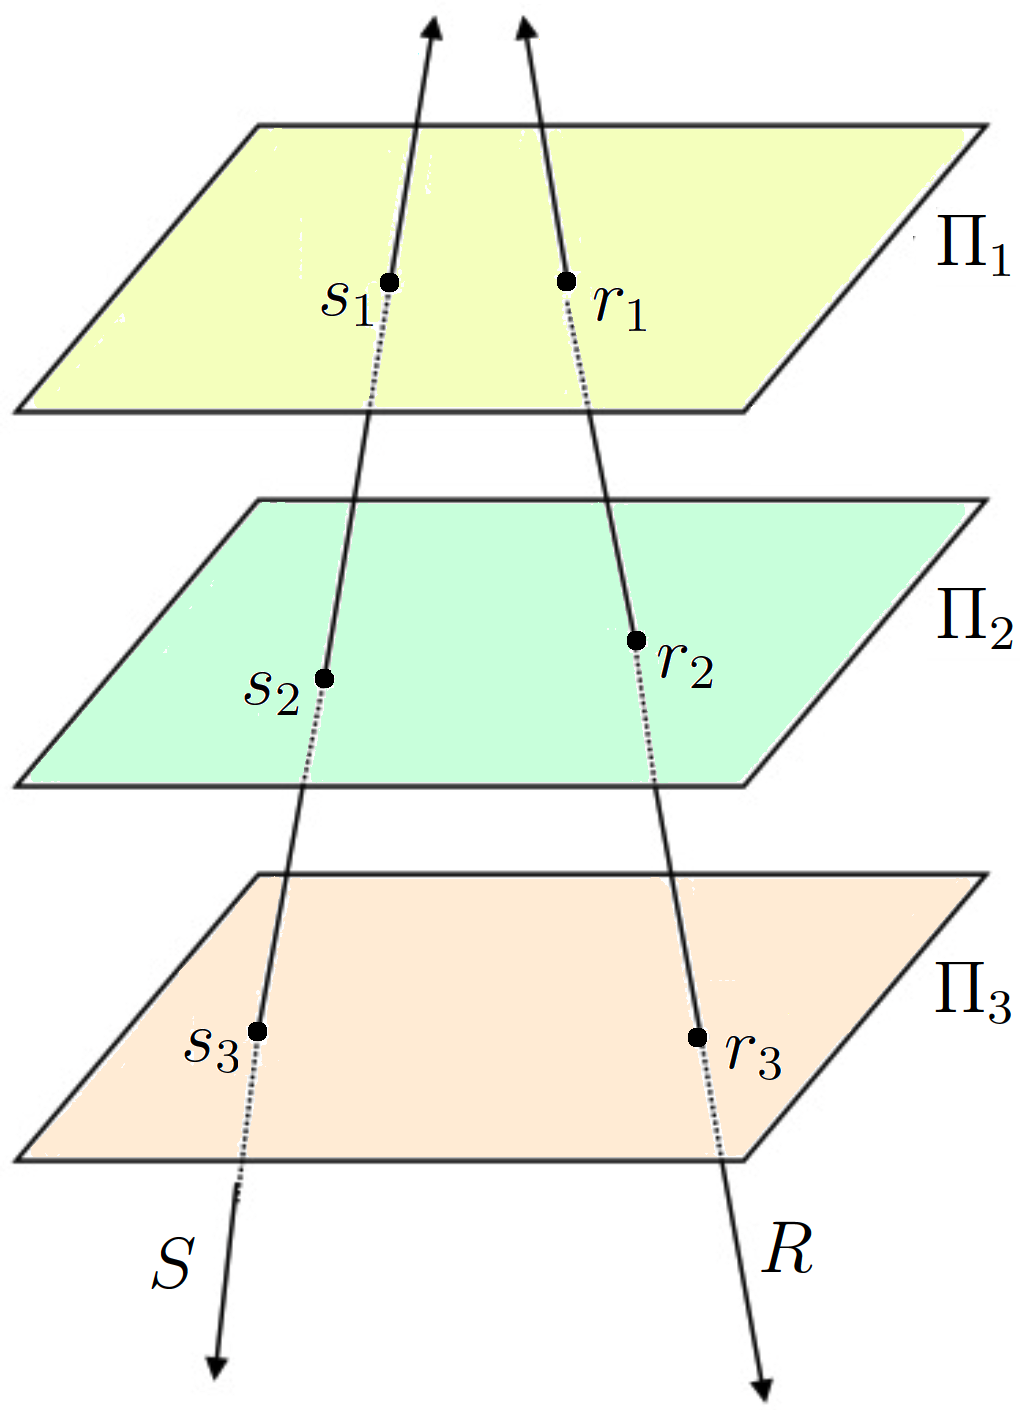
\includegraphics[width=0.3\linewidth]{Thales.png}
        \caption{Teorema de Thales.}
    \end{figure}
\end{teo}
\begin{proof}
    Consideramos $\pi_{S,\Pi_i}$ la proyección afín sobre $S$ paralela a $\Pi_i$ para $i=1,2,3$. Tenemos que:
    \begin{equation*}
        \pi_{S,\Pi_i}(r_j) = s_i + \pi_{\vec{S}, \vec{\Pi}}(\vec{s_ir_j}) = s_i+\vec{s_is_j} = s_j \qquad \forall i,j=1,2,3
    \end{equation*}

    Como $r_1,r_2$ y $r_3$ están alineados, $\exists_1 \lambda\in \bb{R}^\ast$ tal que $\vec{r_1r_3} = \lambda\vec{r_1r_2}$. Por tanto,
    \begin{equation*}
        d(r_1,r_3) = \|\vec{r_1r_3}\| = |\lambda|~\|\vec{r_1r_2}\| = |\lambda|d(r_1,r_2).
    \end{equation*}

    Como $\pi_{S,\Pi_i}$ es afín y $\pi_{S,\Pi_i}(r_j)=s_j$ para $i,j=1,2,3$, tenemos:
    \begin{gather*}
        \vec{\pi}_{S,\Pi_i}(\vec{r_1r_3}) = \vec{\pi_{S,\Pi_i}(r_1)\pi_{S,\Pi_i}(r_3)} = \vec{s_1s_3} \qquad \forall i=1,2,3 \\
        \vec{\pi}_{S,\Pi_i}(\vec{r_1r_2}) = \vec{\pi_{S,\Pi_i}(r_2)\pi_{S,\Pi_i}(r_2)} = \vec{s_1s_2} \qquad \forall i=1,2,3
    \end{gather*}

    Además, como $\vec{\pi}_{S,\Pi_i}$ es lineal, tenemos que:
    \begin{equation*}
        \vec{\pi}_{S,\Pi_i}(\vec{r_1r_3}) = \vec{\pi}_{S,\Pi_i}(\lambda\vec{r_1r_2})
        = \lm\vec{\pi}_{S,\Pi_i}(\vec{r_1r_2}) \Longrightarrow \vec{s_1s_3} = \lm \vec{s_1s_2} \qquad \forall i=1,2,3
    \end{equation*}

    Por tanto,
    \begin{equation*}
        d(s_1,s_3) = \|\vec{s_1s_3}\| = |\lambda|~\|\vec{s_1s_2}\| = |\lambda|d(s_1,_2).
    \end{equation*}

    Por tanto, tenemos que:
    \begin{equation*}
        \frac{1}{|\lm|}=
        \frac{d(s_1, s_2)}{d(s_1,s_3)} = \frac{d(r_1,r_2)}{d(r_1,r_3)}.
    \end{equation*}
\end{proof}


\section{Relación de Ejercicios}

Para ver ejercicios relacionados con este tema, consultar la sección \ref{Rel:Tema2}.